% VLDB template version of 2020-08-03 enhances the ACM template, version 1.7.0:
% https://www.acm.org/publications/proceedings-template
% The ACM Latex guide provides further information about the ACM template
%!TEX program = pdflatex
\documentclass[sigconf, nonacm]{acmart}
%\usepackage{fontspec}
\usepackage{balance}
\usepackage{enumitem}
\usepackage{multirow}
% \usepackage{svg} % For SVG support
\usepackage{graphicx}
\usepackage{ulem}  % 导言区加上这一行
\usepackage{microtype}  %处理换行
\usepackage{subcaption} % 需要subcaption宏包支持子图
% \newtheorem{definition}{DEFINITION} % 定义“定义”环境
% % \newtheorem{example}{例} % 定义“例”环境,不与“定义”共享编号
% %% The following content must be adapted for the final version
% % paper-specific
\newcommand\vldbdoi{XX.XX/XXX.XX}
\newcommand\vldbpages{XXX-XXX}
% issue-specific
\newcommand\vldbvolume{14}
\newcommand\vldbissue{1}
\newcommand\vldbyear{2020}
% should be fine as it is
\newcommand\vldbauthors{\authors}
\newcommand\vldbtitle{\shorttitle} 
% leave empty if no availability url should be set
\newcommand\vldbavailabilityurl{https://github.com/zhujx001/Hybrid-ANNS-Experiment}
% whether page numbers should be shown or not, use 'plain' for review versions, 'empty' for camera ready
\newcommand\vldbpagestyle{plain} 

\begin{document}
	%\begin{sloppypar}
	\title{An Experimental Evaluation of Hybrid Querying on Vectors (EA\&B)}
	
	\author{Jiaxu Zhu}
	\affiliation{%
		\institution{Huazhong University of Science and Technology}
	}
	
	\author{Jiayu Yuan}
	\affiliation{%
		\institution{Huazhong University of Science and Technology}
	}
	
	\author{Kaiwen Yang}
	\affiliation{%
		\institution{Huazhong University of Science and Technology}
	}
	
	\author{Xiaobao Chen}
	\affiliation{%
		\institution{Huazhong University of Science and Technology}
	}
	
	\author{Shihuan Yu}
	\affiliation{%
		\institution{Huazhong University of Science and Technology}
	}
	
	\author{Hongchang Lv}
	\affiliation{%
		\institution{Huazhong University of Science and Technology}
	}
	
	\author{Yan Li}
	\affiliation{%
		\institution{Huazhong University of Science and Technology}
	}
	
	\author{Bolong Zheng}
	\affiliation{%
		\institution{Huazhong University of Science and Technology}
	}
	%%
	%% The "author" command and its associated commands are used to define the authors and their affiliations.
	
	
	% \author{Mengzhao Wang$^1$, Xiaoliang Xu$^1$, Qiang Yue$^1$, Yuxiang Wang$^{1,*}$}
	% \affiliation{%
		%  \institution{$^1$Hangzhou Dianzi University, China}
		% }
	% \email{{mzwang,xxl,yq,lsswyx}@hdu.edu.cn}
	% \author{Ben Trovato$^1$, Lars Th{\o}rv{\"a}ld$^2$, Valerie B\'eranger$^3$, J\"org von \"Arbach$^3$, Wang Xiu Ying$^3$, Donald Fauntleroy Duck$^3$}
	
	% \affiliation{%
		%   \institution{1. Institute for Clarity in Documentation, Ireland}
		%   \institution{2. The Th{\o}rv{\"a}ld Group, Iceland}
		%   \institution{3. Inria Paris-Rocquencourt, France}
		% }
	
	% \email{trovato@corporation.com, larst@affiliation.org, vb@rocquencourt.com, jaerbach@uni-tuebingen.edu, firstname.lastname@ecnu.edu.cn, donald@swa.edu}
	
	%
	% The abstract is a short summary of the work to be presented in the
	% article.
	\begin{abstract}
		Recent studies demonstrate the significant practical value of hybrid queries, which integrate vector search with structured filters (e.g., attribute and range filtering) for refined retrieval.
		However, current evaluations lack unified benchmarking standards and systematic assessment methodologies. Existing studies not only fail to cover mainstream algorithms but also omit systematic comparisons or in-depth analysis on different methods. To address this issue, we design a complete evaluation framework for hybrid queries. Our study introduces 15 hybrid query algorithms and systematically classifies them based on multiple dimensions, such as index organization and filtering strategy, providing a reference for the categorization of hybrid queries. In experiments, for attribute filtering, we construct standard attribute sets, enabling a unified comparison of algorithms in terms of index construction efficiency, query performance, and robustness. For range filtering, we also evaluate the algorithm performance across the 3 metrics through controlled variation of query ranges. Additionally, we conduct an in-depth analysis of the experimental results based on the underlying principles of algorithms. Extensive experimental results reveal the strengths and weaknesses of each algorithm. Based on the findings, we develop a set of practical guidelines for algorithm selection, offering reliable references for different application scenarios. Furthermore, we identify potential directions for improvement to address the current limitations of these algorithms.
		
	\end{abstract}
	
	
	\maketitle
	
	%%% do not modify the following VLDB block %%
	%%% VLDB block start %%%
	\pagestyle{\vldbpagestyle}
	\begingroup\small\noindent\raggedright\textbf{PVLDB Reference Format:}\\
	\vldbauthors. \vldbtitle. PVLDB, \vldbvolume(\vldbissue): \vldbpages, \vldbyear.\\
	\href{https://doi.org/\vldbdoi}{doi:\vldbdoi}
	\endgroup
	\begingroup
	\renewcommand\thefootnote{}\footnote{\noindent
		This work is licensed under the Creative Commons BY-NC-ND 4.0 International License. Visit \url{https://creativecommons.org/licenses/by-nc-nd/4.0/} to view a copy of this license. For any use beyond those covered by this license, obtain permission by emailing \href{mailto:info@vldb.org}{info@vldb.org}. Copyright is held by the owner/author(s). Publication rights licensed to the VLDB Endowment. \\
		\raggedright Proceedings of the VLDB Endowment, Vol. \vldbvolume, No. \vldbissue\ %
		ISSN 2150-8097. \\
		\href{https://doi.org/\vldbdoi}{doi:\vldbdoi} \\
	}\addtocounter{footnote}{-1}\endgroup
	%%% VLDB block end %%%
	
	%%% do not modify the following VLDB block %%
	%%% VLDB block start %%%
	\ifdefempty{\vldbavailabilityurl}{}{
		
		\begingroup\small\noindent\raggedright\textbf{PVLDB Artifact Availability:}\\
		The source code, data, and/or other artifacts have been made available at \url{\vldbavailabilityurl}.
		\endgroup
	}
	%%% VLDB block end %%%
	
	\section{Introduction}
	
	Nearest Neighbor (NN) search \cite{cover1967nearest} aims to find the closest vector in a given space and serves as a fundamental algorithm in vector retrieval, with widespread applications in recommendation systems  \cite{monolith}  and image retrieval \cite{wang2012scalable}.
	% 需要添加引用,下面这段
	However, with the exponential growth of data volume and the increasing dimensionality of vectors \cite{weber1998quantitative}, traditional NN search methods struggle to meet the demands of real-time search. To address this issue, studies turn to more efficient approaches - Approximate NN (ANN) search ~\cite{arya1998optimal,beis1997shape,gionis1999similarity,malkov2018efficient}, which significantly improve search efficiency by constructing effective indexing structures, albeit at the cost of reduced accuracy.
	
	Nevertheless, as application scenarios grow increasingly complex, simple ANN search can no longer satisfy all practical needs. For instance, Fig.~\ref{fig:hybrid ANNS} illustrates a case where users on e-commerce platforms search for clothing items by retrieving visually similar products based on an image. Additionally, users may impose further requirements such as price, color, or brand preferences. Such scenarios necessitate a retrieval system capable of simultaneously addressing vector similarity (e.g., product image) and attribute constraints (e.g., brand name) \cite{tian2023approximate}. When the constraint involves a specific attribute value, this problem refers to Attribute Filtering Approximate Nearest Neighbor (AF-ANN) search ~\cite{NHQ,Filtered-diskann} . For example, a user may seek a green piece of clothing. If the constraint involves a range condition, the problem is known as Range Filtering Approximate Nearest Neighbor (RF-ANN) search ~\cite{serf,iRangeGraph}. For instance, filtering clothes priced between 100 and 200. To meet these application demands, hybrid querying \cite{JD-e-commerce, analyticdb} techniques emerge. Hybrid queries integrate vector retrieval with conditional filtering, optimizing their interaction to significantly enhance efficiency and flexibility in complex query scenarios.
	
	\begin{figure*}
		\centering
		
		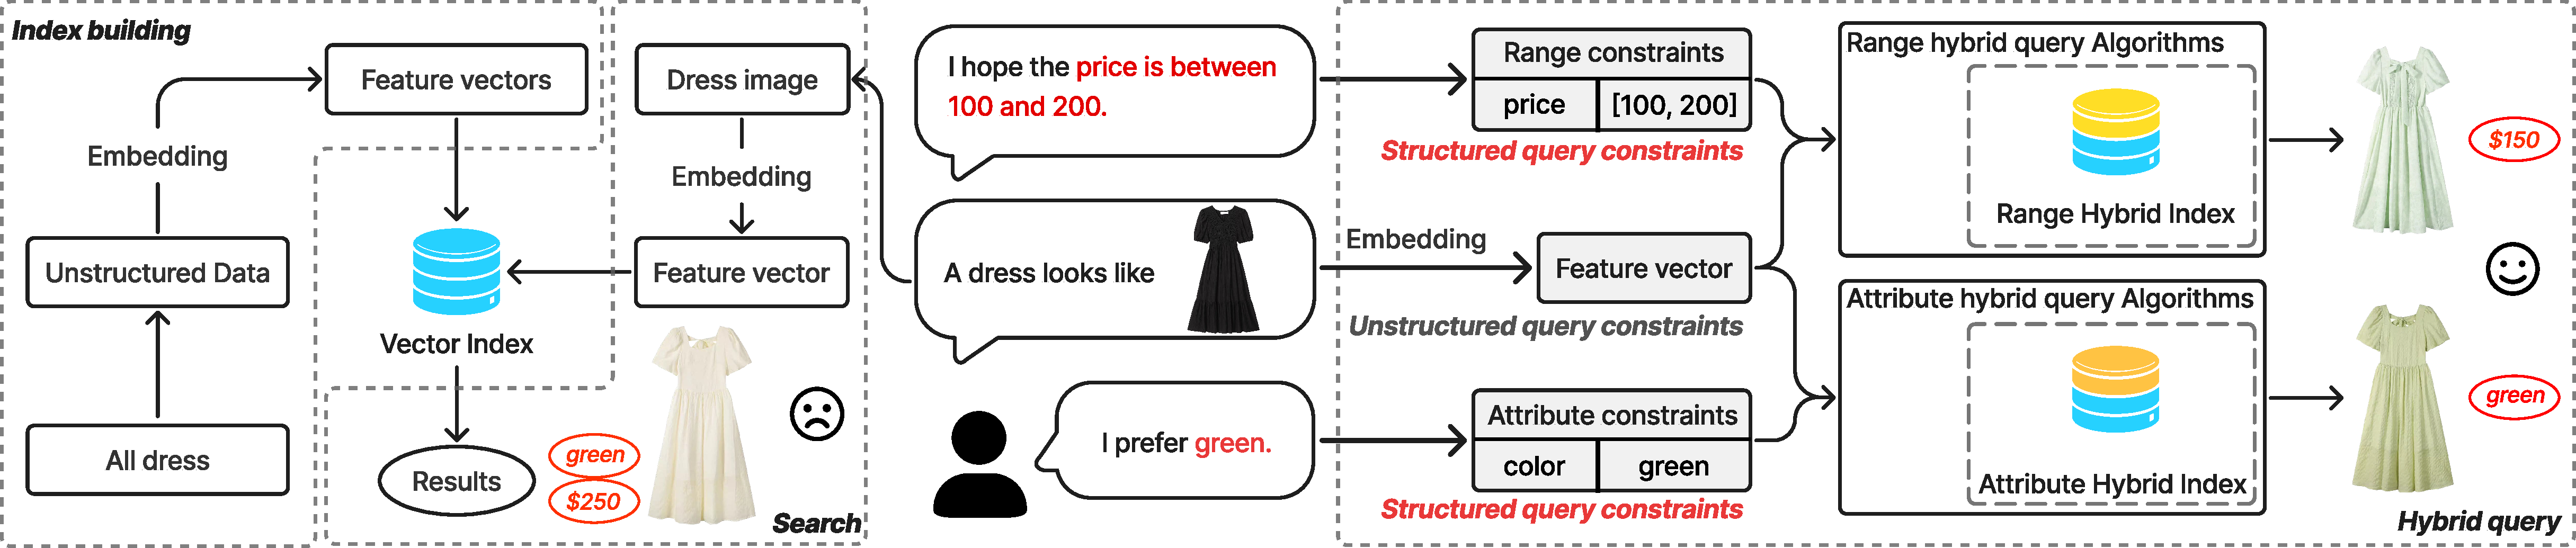
\includegraphics[width=0.92\textwidth]{figures/hybrid ANNS.pdf}
		\caption{Hybrid query example}
		
		\label{fig:hybrid ANNS}
	\end{figure*}
	\subsection{Motivation}
	
	In recent years, hybrid query algorithms develop rapidly, giving rise to numerous attribute filtering ~\cite{NHQ,diskann} and range filtering algorithms \cite{serf,iRangeGraph}. In practical applications, the performance of hybrid query algorithms is influenced not only by unstructured data but also closely related to structured data. For attribute filtering algorithms, factors such as the number of attributes, attribute distribution \cite{UNG}, and attribute selectivity \cite{ACORN} significantly impact algorithm performance. As for range filtering algorithms, the size of the query range and the characteristics of different datasets  play an important role in determining algorithm performance.
	
	Despite BigANN 2023 \cite{bigann2023} evaluates the performance of some ANN algorithms, it presents several notable limitations:
	1) The evaluation covers a limited number of algorithms and fails to comprehensively include mainstream methods. 
	%	\sout{For instance, attribute filtering algorithms such as NHQ and UNG are not included in the evaluation. }
	2) It focuses only on single-attribute and dual-attribute query scenarios. 
	%	\sout{neglecting the more complex demands of multi-attribute queries. In real-world applications, an object typically involves multiple attributes.}\textcolor{blue}{ \sout{For example, in e-commerce scenarios, users often specify multiple attributes (e.g., color, brand, price range) simultaneously when searching.}}
	3) It does not evaluate algorithm performance under different attribute distributions. 
	%	\sout{However, variations in attribute distribution may directly affect the filtering strategies and index construction efficiency of hybrid query algorithms.}
	
	Moreover, beyond BigANN, systematic evaluations of hybrid query algorithms remain limited. To fill this gap, we conduct a comprehensive experimental evaluation of hybrid query algorithms, analyzing the index construction costs and query efficiency across different scenarios. Additionally, we further assess the robustness of each algorithm under varying conditions.
	
	
	\subsection{Our Contributions}
	
	Our study focuses on the problem of ANN search in hybrid query scenarios and provides a comprehensive review and evaluation of existing algorithms and systems. The main contributions are summarized in the following 5 aspects.
	
	(1)\textbf{ Systematic Classification and Overview.}
	%We systematically classify 6 representative attribute filtering algorithms from multiple dimensions, including index organization, filtering strategy, Boolean logic support, and index construction methods. Additionally, we survey 5 range filtering algorithms and provide an overview of widely used vector retrieval libraries (e.g., Faiss) and vector databases (e.g., Milvus, PASE, VBASE). These efforts provide a unified reference framework for future study.
	We systematically classify 6 representative attribute filtering algorithms along multiple dimensions, including index organization, filtering strategies, Boolean logic support, and index construction methods. In addition, we survey 5 range filtering algorithms, and provide an overview of a vector retrieval library and three vector databases. These efforts offer a unified reference framework for future research.
	
		(2) \textbf{Enhancing Datasets and Experimental Settings for Fair Evaluation.}
		To address the lack of standardized benchmarks in attribute filtering research, we enrich commonly used datasets by generating attribute values tailored to real-world scenarios. Furthermore, we design comprehensive experimental settings that reflect diverse application requirements, including varying attribute distributions, selectivity, and query conditions. These enhancements provide a unified evaluation framework that supports fair, consistent, and reproducible comparisons across different algorithms, laying a solid foundation for future research in hybrid query.
	
	
	(3)\textbf{ Evaluation of Attribute Filtering Algorithms.}
	%We conduct a systematic evaluation of 13 attribute filtering algorithms on 7 real-world datasets. 
	We systematically evaluate 6 attribute filtering algorithms, 1 library, and 3 databases on 7 real-world datasets. By analyzing performance under varying numbers of attributes, we reveal the strengths and weaknesses of each method. We further examine their behavior under different attribute distributions and selectivity to assess robustness and adaptability in complex query scenarios. Evaluation metrics include index construction time, index size, peak memory usage, QPS, and search accuracy.
	
	(4)\textbf{ Evaluation of Range Filtering Algorithms.}
	%We benchmark 5 range filtering algorithms\textcolor{red}{, 1 library, and 3 databases} 
	We benchmark algorithms that support range filtering on 3 large-scale datasets, using varying query range settings in the experiments. The experimental results show the performance of these algorithms in terms of index construction efficiency, storage overhead, and query performance. We further analyze the factors that affect the performance of the range query algorithm.
	
	
	(5)\textbf{ Recommendations and Challenges.}
	Based on the experimental results, we provide algorithm selection recommendations for common application scenarios and highlight key challenges in the field of hybrid queries. These challenges include limited Boolean logic support, the lack of multi-attribute range filtering capabilities, and the sensitivity of algorithms to data distribution. Currently, few methods simultaneously support both attribute filtering and range filtering, pointing to potential directions for future research.
	
	\section{PRELIMINARIES}
	
	\subsection{Problem Definition}
	
	We first define the Nearest Neighbor (NN) search problem.
	
	\begin{definition}[NN Search]
		
		Let \( D = \{v_1, \ldots, v_n\} \) be a dataset of \( n \) \( d \)-dimensional vectors. Given a query \( Q = (q_v, k) \), where \( q_v \) is the query vector and \( k \) is a positive integer, the NN search aims to return a set \( R \subseteq D \) with \( |R| = k \), such that for any \( x \in R \) and \( y \in D \setminus R \), \( \textit{dist}\!\left(q_v, x\right) \leq \textit{dist}\!\left(q_v, y\right) \). Here, \( \textit{dist}\!\left(\cdot, \cdot\right) \) denotes the distance metric, and we adopt Euclidean distance in this paper.
	\end{definition}
	
	However, to address the curse of dimensionality faced by NN search \cite{dimcurse}, existing studies focus on approximate solutions, known as ANN  search. We typically use $\text{Recall}@k = \frac{|R \cap \hat{R}|}{k}$ to evaluate the accuracy of ANN search algorithms, where $R$ denotes the true top-$k$ nearest neighbors of the query, and $\hat{R}$ denotes the approximate top-$k$ nearest neighbors returned by the ANN search algorithm.
	
	As the complexity of real-world application requirements increases, NN search has evolved into hybrid NN search with attribute constraints. Depending on the nature of the attribute constraints, hybrid NN search can be divided into 2 categories: 1) Attribute Filtering Nearest Neighbor (\textit{AF-NN}) search. 2) Range Filtering Nearest Neighbor (\textit{RF-NN}) search. We provide their formal definitions below.
	
	\begin{definition}[AF-NN Search]
		Let \( D = \{(v_1, s_1), \ldots, (v_n, s_n)\} \) be a dataset of \( n \) \( d \)-dimensional vectors, each associated with an attribute set \( s_i \). Given a query \( Q = (q_v, q_s, k) \), where \( q_s \) is the query attribute set, the AF-NN search aims to return a set \( R \subseteq D_s \) with \( |R| = k \), such that for any \( x \in R \) and \( y \in D_s \setminus R \), \( \textit{dist}(q_v, x) \leq \textit{dist}(q_v, y) \), where \( D_s = \{ v_i \mid (v_i, s_i) \in D \land q_s \subseteq s_i \} \).
	\end{definition}
	
	%	We further classify AF-NN search according to the number of the attribute set \( s_i \): 1) Single-Attribute Filtering Nearest Neighbor (\textit{SAF-NN}) search, where $\forall i,\, |s_i| = 1$. 2) Multi-Attribute Filtering Nearest Neighbor (\textit{MAF-NN}) search, where $\exists i,\, |s_i| > 1$.
	
	\begin{definition}[RF-NN Search]
		
		Let \( D = \{(v_1, a_1), \ldots, (v_n, a_n)\} \) be a dataset of \( n \) \( d \)-dimensional vectors, each associated with an attribute value \( a_i \). Given a query \( Q = (q_v, [a_{\min}, a_{\max}], k) \), where \( a_{\min} \) and \( a_{\max} \) denote the lower and upper bounds of the query range, respectively, the RF-NN search aims to return a set \( R \subseteq D_a \) with \( |R| = k \), such that for any \( x \in R \) and \( y \in D_a \setminus R \), \( \textit{dist}(q_v, x) \leq \textit{dist}(q_v, y) \), where \( D_a = \{ v_i \mid (v_i, a_i) \in D \land a_{\min} \leq a_i \leq a_{\max} \} \).
	\end{definition}
	
	
	
	Similar to the conventional ANN search, most existing studies focus on approximate solutions for hybrid NN search, referred to as hybrid ANN search, which includes both \textit{AF-ANN} search and \textit{RF-ANN} search.
	
	
	
%	\subsection{Index Organization in Hybrid ANN Search}
	\subsection{Index Organization in Hybrid Query}
	
	Current hybrid query methods mainly adopt graph-based ~\cite{nsw,kgraph,nsg,fanng,ngt} or Inverted File Index (IVF)-based \cite{PQ} index organization. 
	%We briefly introduce the fundamental principles of these two types in the following.
	\textcolor{violet}{Here, we briefly review the core concepts of these indexes and outline how attributes and range constraints are embedded to support hybrid query functionality.}
	
	\noindent\textbf{\underline{Graph.}}
	Graph-based ANN search algorithms accelerate queries by building graph indexes on datasets. As illustrated in Figure~\ref{fig:graph}, each data point in the dataset corresponds to a point in the graph, and neighboring vertices (e.g., $a$ and $b$) are connected via edges based on their distance $\textit{dist}(a, b)$. In the graph index, each point maintains connections only to its nearest neighbors to preserve query efficiency. For instance, in Figure~\ref{fig:graph}, the gray point $c$ is connected to 5 neighbors $(a, b, d, e, f)$ and can traverse to them via corresponding edges.
	
	Given a query point $q$, the graph-based ANN search typically follows a greedy search strategy to find the $k$ nearest neighbors. For illustration, consider the case where $k = 1$ (i.e., 1NN): The algorithm initiates the search from an entry point (the gray point $c$). If there exists a neighbor $n$ (the point $f$) of the current point such that $\textit{dist}(n, q) < \textit{dist}(c, q)$, the algorithm updates the current point to $n$. This process is iteratively repeated—always moving to the neighbor closest to $q$—until no neighbor is found that is closer than the current point. The final point reached (the blue point $j$) is returned as the approximate nearest neighbor of $q$.
	
	\textcolor{violet}{Graph-based indexes are widely adopted in Hybrid ANN search algorithms due to their excellent performance. To support hybrid queries, existing approaches usually augment the original graph structures by explicitly associating attribute or range information with vertices or edges. In attribute filtering, a common approach is to attach attribute metadata to vertices or edges, allowing the traversal process to skip nodes or edges that do not meet the query's attribute conditions (e.g., NHQ, Filtered-DiskANN, ACORN). In range filtering, edges typically store valid attribute intervals, and traversal proceeds only along edges satisfying the range constraints, effectively narrowing down the search space (e.g., SeRF, DSG).}
	
	
	\noindent\textbf{\underline{IVF.}}  IVF-based ANN search algorithms improve computational efficiency by partitioning the dataset into clusters and restricting the search to clusters nearest to the query point. Specifically, as shown in Figure~\ref{fig:ivf}, IVF first selects a subset of data points and applies a clustering algorithm (e.g., K-Means) to obtain a set of centroids $(C_0, C_1, ..., C_6)$, each representing a distinct cluster. Every data point (gray dots) is then assigned to the cluster corresponding to its nearest centroid based on the distance metric, thereby forming the index structure.
	
	During the query process, given a query point $q$, the algorithm computes distances between $q$ and all centroids, selects a small number of the closest centroids ($C_0, C_1, C_2$), and then performs a search only within the associated clusters to identify the approximate nearest neighbors.
	
	\textcolor{violet}{IVF-based indexes also offer unique advantages in Hybrid ANN search scenarios, such as naturally supporting pre-filtering and requiring significantly lower memory consumption and smaller index sizes compared to graph-based indexes. With minor modifications, IVF indexes achieve attribute and range filtering by directly excluding vectors that do not meet query constraints through pre-filtering, thus skipping irrelevant vectors during intra-cluster distance computations (e.g., Faiss, Milvus). Moreover, clusters can be further partitioned hierarchically based on attributes (hierarchical partitioning), resulting in finer-grained sub-partitions that significantly enhance the efficiency of attribute filtering (e.g., CAPS, PUCK).}
	
	\begin{figure}
		\begin{subfigure}{0.60\columnwidth}
			\centering
			
			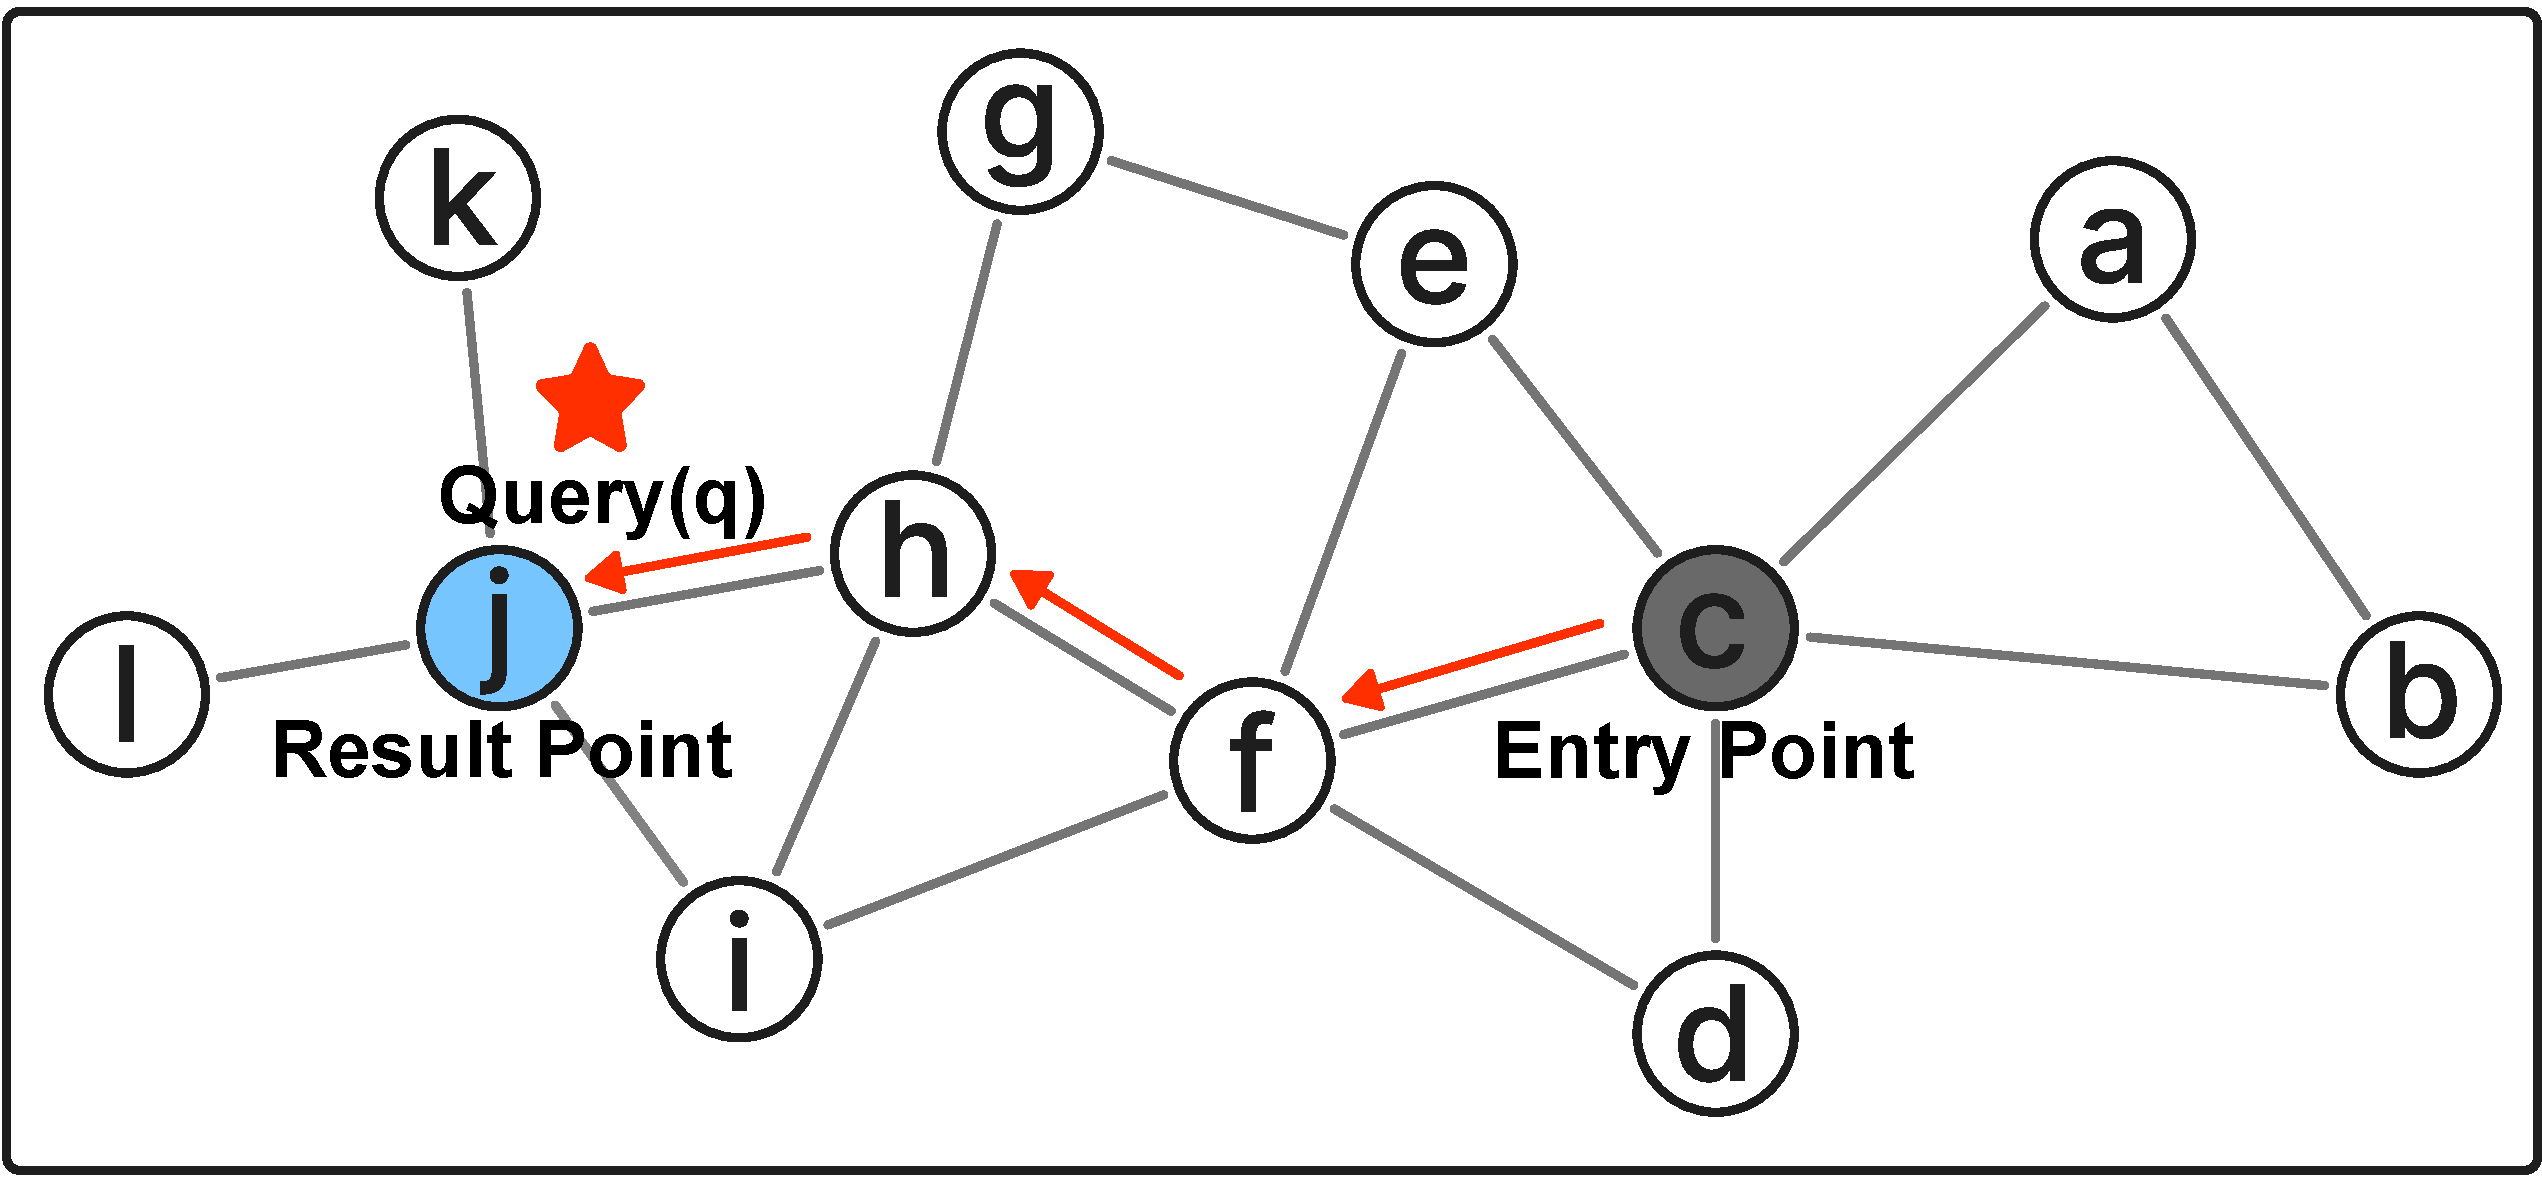
\includegraphics[width=\linewidth]{figures/graph.pdf}
			\caption{Graph Index}
			\label{fig:graph}
		\end{subfigure}
		\hfill
		\begin{subfigure}{0.38\columnwidth}
			\centering
			
			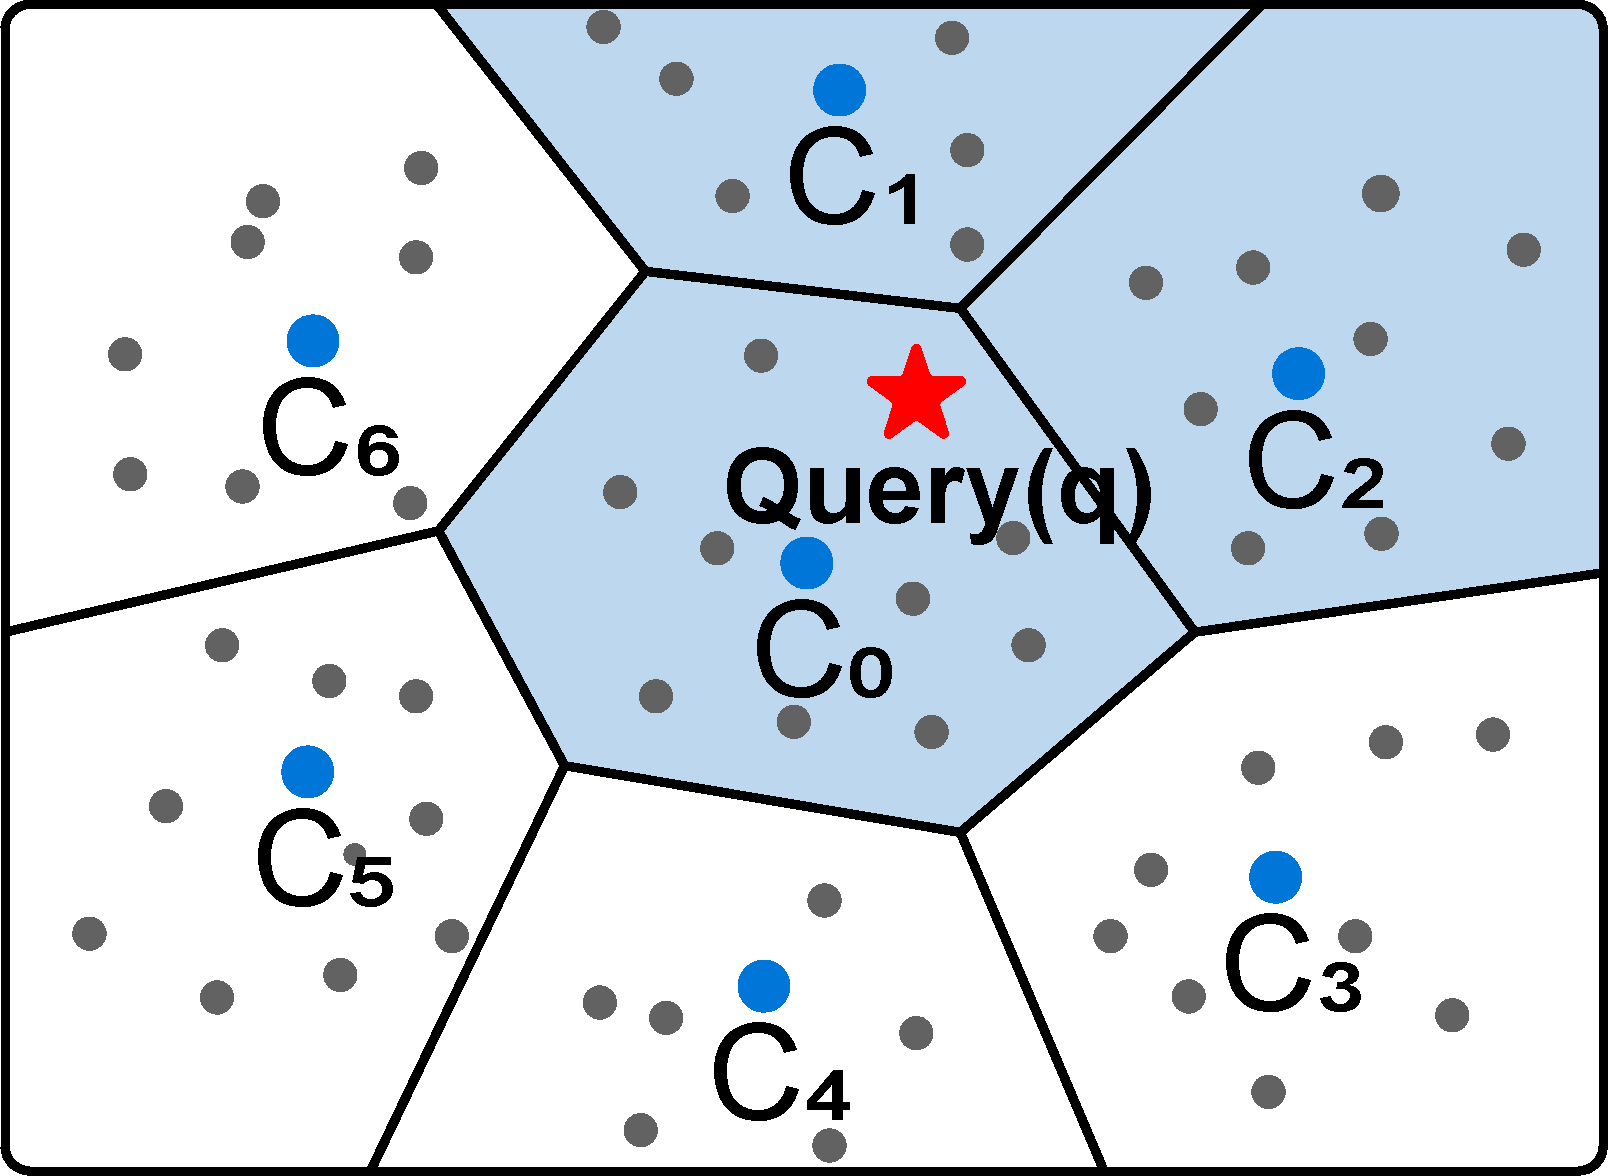
\includegraphics[width=\linewidth]{figures/ivf.pdf}
			\caption{IVF Index}
			\label{fig:ivf}
		\end{subfigure}
		
		
		\caption{Graph index and IVF index}
		
	\end{figure}
	
	
	\section{Hybrid query Algorithms}
	
	
	\renewcommand{\arraystretch}{0.9}
	\begin{table*}[t]
		\centering
		%\setlength{\belowcaptionskip}{-0.3cm}
		
		\caption{Comparison of AF-ANN search algorithms}
		\small
		\label{tab:compair_1}
		\begin{tabular}{|l|l|c|c|c|c|c|c|c|}
			\hline
			\textbf{Algorithm} & \textbf{Base} & \textbf{Filter Type} & \textbf{AND} & \textbf{OR} & \textbf{Flexible Attributes} & \textbf{Complex Boolean} & \textbf{Dynamic Insert} & \textbf{Multi Thread} \\
			\hline
			NHQ & Graph & C & Y & N& N& N & N & N \\
			FilteredVamana & Graph & C & N & Y & Y & N & Y & Y \\
			StitchedVamana & Graph & C & N & Y & Y & N & N & Y  \\
			CAPS & IVF & C & Y & N & Y & N & Y & Y \\
			ACORN & Graph & B & Y & Y & Y & Y & Y & Y \\
			UNG & Graph & B & Y & Y & Y & N & Y & Y \\ 
			Puck & IVF & B & Y & Y & Y & N & Y & Y \\
			% ParlayANN & Graph+IVF & B & N & N & Y & N & N & Y \\
			
			\hline
			
		\end{tabular}
		
		
		\centering
		%	 \setlength{\abovecaptionskip}{0cm}
		%	\setlength{\belowcaptionskip}{0.1cm}
		\footnotesize{
			\begin{minipage}{\linewidth}
				\vspace{0.1cm}
				\textsuperscript{A} Post-filtering, 
				\textsuperscript{B} Pre-filtering, 
				\textsuperscript{C} Simultaneous filtering, 
				\textsuperscript{Y} Support, 
				\textsuperscript{N} Unsupport. 
				\textit{Base} indicates that the hybrid query algorithm is an improvement based on a specific ANN search algorithm. 
				\textit{AND} indicates whether the algorithm supports attribute filtering with AND operations. 
				\textit{OR} indicates whether the algorithm supports attribute filtering with OR operations. 
				\textit{Flexible Attributes} indicates whether the number of query attributes can differ from the number of attributes used during index construction. 
				\textit{Complex Boolean} refers to whether the algorithm supports advanced Boolean logic beyond just AND and OR, such as NOT or combinations like (A AND B) OR (C AND NOT D). 
				\textit{Dynamic Insert} indicates whether the algorithm supports the operation of dynamically inserting data points.
				\textit{Multi Thread} indicates whether the algorithm supports multi-threaded search.
		\end{minipage}}
		
	\end{table*}
	
	
	%We provide an overview and analysis of 15 hybrid query methods, all drawn from recent studies, and collectively referred to as algorithms in the following. Specifically, Section~3.1 describes methods for attribute filtering, Section~3.2 discusses those for range filtering, and Section~3.3 introduces vector libraries and databases that support both attribute filtering and range filtering.
	
	
	\subsection{Attribute Filtering Algorithms}
	
	We summarize 6 attribute filtering algorithms and provide an intuitive comparison in Table~\ref{tab:compair_1}.

%	\noindent\textbf{\underline{NHQ \cite{NHQ}.}}  
%	\footnote{https://github.com/KGLab-HDU/TKDE-under-review-Native-Hybrid-Queries-via-ANNS}
	\noindent\textbf{\underline{NHQ} \footnote{https://github.com/KGLab-HDU/TKDE-under-review-Native-Hybrid-Queries-via-ANNS} \cite{NHQ}}
	Traditional attribute filtering algorithms usually perform attribute constraints and ANN search separately. In contrast, NHQ is the first to implement simultaneous filtering, integrating both aspects into a unified framework. NHQ constructs an index based on a nearest neighbor graph and introduces a fusion distance that jointly captures vector similarity and attribute similarity. Leveraging this fusion distance, NHQ unifies vector similarity and attribute matching into a single comprehensive similarity measure and builds the graph accordingly. During the query process, NHQ efficiently prunes irrelevant edges via this composite index, enabling fast retrieval of results that satisfy both vector similarity and attribute constraints.
	
	\noindent\textbf{\underline{Filtered-DiskANN} \footnote{https://github.com/microsoft/DiskANN} \cite{Filtered-diskann}}
	%\sout{The effectiveness of NHQ may degrade when the number of attributes changes, as it affects the fusion distance computation. Filtered-DiskANN addresses this limitation.}
	Filtered-DiskANN also supports simultaneous filtering. Built upon the Vamana \cite{diskann} graph-based ANN index, it incorporates attribute information directly into the graph during index construction. This integration ensures that the index reflects both vector similarity and attribute constraints. Moreover, Filtered-DiskANN supports SSD-based storage, improving scalability.
	Filtered-DiskANN proposes 2 indexes:  
	1) \textbf{FilteredVamana}, which incrementally builds the graph index by inserting data points and dynamically adding edges, allowing adaptive expansion.  
	2) \textbf{StitchedVamana}, which adopts a batch construction strategy—constructing separate Vamana subgraphs for each attribute, followed by merging and edge pruning.
	%	A key limitation of Filtered-DiskANN is that only supports the Boolean OR logic for multi-attribute filtering, lacking support for Boolean AND logic.
	
	
	\noindent\textbf{\underline{CAPS} \footnote{https://github.com/gaurav16gupta/constrainedANN} \cite{CAPS}}
	%\sout{Different from the above graph-based simultaneous filtering algorithms,}
	CAPS is the first simultaneous filtering algorithm based on spatial partitioning.
	It introduces a hierarchical sub-partitioning algorithm inspired by Huffman trees, termed the Attribute Frequency Tree (AFT), to overcome the coarse granularity of traditional IVF-based methods. CAPS adopts a two-level partitioning strategy:  
	1) The first level clusters vectors based on similarity using K-Means or learning-based methods such as BLISS. 2) Within each cluster, AFT partitions data further based on attribute frequencies, enabling finer-grained indexing and improving query efficiency.
	
	\noindent\textbf{\underline{ACORN} \footnote{https://github.com/stanford-futuredata/ACORN} \cite{ACORN}}
	%	Above simultaneous filtering algorithms struggle with large-scale, unbounded, or unknown predicate sets.
	%	%The above simultaneous filtering methods are less effective in scenarios involving large-scale, unbounded, or unknown predicate sets, where a predicate refers to a condition or rule used for filtering. 
	%	ACORN addresses this issue by introducing a predicate-agnostic indexing framework.
	%	ACORN is built upon Hierarchical Navigable Small World (HNSW) \cite{hnsw}. It supports high-cardinality and unrestricted predicate sets, overcoming the limitations of methods restricted to small-scale equality filters. It constructs a denser hierarchical graph by expanding node neighborhoods and prunes edges at lower levels to control index size. During the query process, ACORN eliminates unnecessary distance computations by filtering out nodes that violate attribute constraints. This effectively maintains a nearest neighbor graph over valid nodes only. 
	%	%During the query process, ACORN avoids unnecessary distance computations by filtering out nodes that do not meet attribute constraints, effectively simulating a nearest neighbor graph over valid nodes only.
	%	ACORN includes 2 indexes: 1) \textbf{ACORN-$\gamma$}, which expands neighbor lists during construction, increasing memory usage for higher performance.  
	%	2) \textbf{ACORN-1}, which extends neighbor lists by considering second-hop neighbors during search, reducing index size with minor performance loss.
	%Above simultaneous filtering algorithms struggle with large-scale, unbounded, or unknown predicate sets. ACORN addresses this by introducing a predicate-agnostic indexing framework.
	Pre-filtering methods apply attribute constraints prior to ANN search. As a pre-filtering approach, ACORN adopts a predicate-agnostic indexing framework to overcome the limitations of the aforementioned simultaneous filtering methods in handling large-scale or unknown predicate settings.
	Based on Hierarchical Navigable Small World (HNSW) \cite{hnsw}, ACORN constructs a denser hierarchical graph with neighborhood expansion and edge pruning. During search, it filters out nodes violating constraints, maintaining a valid nearest neighbor graph.
	ACORN includes two indexes: 1) \textbf{ACORN-$\gamma$}, which expands neighbor lists during construction, trading memory for higher performance; 
	2) \textbf{ACORN-1}, which extends neighbor lists via second-hop neighbors during search, reducing index size with minor performance loss.
	
	\noindent\textbf{\underline{UNG} \footnote{https://github.com/YZ-Cai/Unified-Navigating-Graph} \cite{UNG}} 
	%\sout{The above simultaneous filtering algorithms may not guarantee the completeness of the results and perform poorly when the attribute selectivity is low. UNG is proposed to overcome these limitations.It is a unified framework that integrates diverse graph-based ANN indexes for hybrid query.}
	Similar to ACORN, UNG adopts a pre-filtering strategy and serves as a unified framework that integrates various graph-based ANN indexes to support hybrid queries. It first groups the dataset by attribute sets, ensuring that vectors in each group share identical attributes. Then, it constructs a Label Navigating Graph (LNG) to encode inclusion relationships among attribute sets. Within each group, UNG builds graph-based ANN indexes (e.g., Vamana, HNSW) and connects them via cross-group edges to enable efficient cross-group search.
	%UNG supports Boolean filtering with 2 modes:  1) The query attribute set is a subset of the data attribute set.  2) The query attribute set exactly matches the data attribute set.
	
	
	
	\noindent\textbf{\underline{Puck} \footnote{https://github.com/baidu/puck} \cite{puck}} 
	%While simultaneous filtering algorithms perform well in most scenarios, it may underperform when only a small portion of data satisfies attribute constraints. In such cases, a pre-filtering strategy—applying attribute constraints prior to ANN search—can be more effective.
	Puck also adopts a pre-filtering strategy. Developed by Baidu, Puck utilizes two-level quantization for indexing. It maintains an attribute set for each cluster to track vector attributes. During the query process, it employs pre-filtering to exclude clusters without required attributes, thereby reducing the search space.
	%Developed by Baidu, Puck adopts a pre-filtering approach and employs a multi-level filtering mechanism for hybrid query. Its index structure comprises four layers: the first two use vector quantization for training, while the latter two leverage product quantization.
	
	
	
	\renewcommand{\arraystretch}{0.9}
	\begin{table}[t]
		\centering
		
		\setlength{\textfloatsep}{0.1cm}
		\caption{Comparison of RF-ANN search algorithms}
		\small	% 只会影响当前组的内容
		\label{tab:range_algo}
		\begin{tabular}{|c|c|c|c|}
			\hline
			\textbf{Algorithm} & \textbf{Base} & \textbf{Dynamic Insert} & \textbf{Multi Thread} \\
			\hline
			DSG & Graph & Y & N \\
			iRange & Graph & N & Y \\
			SeRF & Graph & Y & Y \\
			UNIFY & Graph & Y & Y \\
			WinFilter & Graph & N & Y  \\
			\hline
		\end{tabular}
		
		
		\footnotesize{
			\begin{minipage}{\linewidth}
				\centering
				The indicators are consistent with those in Table ~\ref{tab:compair_1}.
				%				\textsuperscript{Y} Support, 
				%				\textsuperscript{N} Unsupport.
				%				\textit{Base} indicates that the hybrid query algorithm is an improvement based on a specific ANN search algorithm. 
				%				\textit{Dynamic Insert} indicates whether the algorithm supports the operation of dynamically inserting data points.
				%				\textit{Multi Thread} indicates whether the algorithm supports multi-threaded search.
			\end{minipage} 
			
		}
		
	\end{table}
	
	\subsection{Range Filtering Algorithms}
	
	We introduce 5 representative range filtering algorithms and present a comparative overview in Table~\ref{tab:range_algo}.
	
	\noindent\textbf{\underline{SeRF} \footnote{https://github.com/rutgers-db/SeRF} \cite{serf}} Conventional RF-ANN search approaches typically follow one of two paradigms: 1) Conducting ANN search first followed by attribute-based filtering. 2) Filtering the dataset based on attribute ranges before performing ANN search. Building a separate neighbor graph (e.g., HNSW) for each attribute range could ensure efficient querying but incurs an $O(n^2)$ cost in constructing and storing $n$ graphs. Since many edges are shared across these graphs, SeRF introduces a validity-range aware design where each edge records the interval in which it is valid, indicating in which subgraphs the edge remains valid. This compresses $n$ graphs into a single unified graph, maintaining search effectiveness while significantly reducing memory and index construction overhead.
	
	\noindent\textbf{\underline{WinFilter} \footnote{https://github.com/JoshEngels/RangeFilteredANN} \cite{winFilter}}
	Unlike SeRF, which focuses on graph compression, WinFilter proposes a structural partitioning framework called the $\beta$-Window Search Tree ($\beta$-WST). After the dataset is sorted by attribute values, it is partitioned into multiple intervals and organized into a tree structure. Each node in the tree corresponds to an attribute range and maintains a local ANN index (e.g., Vamana). For a range filtering query, WinFilter only searches within nodes overlapping the query range and merges partial results. With a tree height of $O(\log n)$, each query accesses at most $O(\log n)$ sub-indexes, resulting in significant speedups.
	
	\noindent\textbf{\underline{iRange} \footnote{https://github.com/YuexuanXu7/iRangeGraph} \cite{iRangeGraph}}
	To address the query efficiency degradation caused by the graph compression in SeRF, iRange adopts a more flexible strategy.
	%Rather than prebuilding indexes for all possible ranges, it dynamically assembles a query-specific subgraph at runtime.
	iRange partitions the dataset into intervals based on attribute values and independently constructs a local graph for each interval, storing only edge information. During the query process, the relevant local graphs overlapping with the query range are merged into a temporary search graph, and a pruning strategy is applied to enable efficient search.
	
	\noindent\textbf{\underline{DSG} \footnote{https://github.com/rutgers-db/DynamicSegmentGraph} \cite{DSG}}
	Most RF-ANN search methods, such as iRange and WinFilter, are designed for static datasets. SeRF allows incremental insertion but requires ordered attributes. DSG introduces the first dynamic RF-ANN framework supporting data insertion with unordered attributes while maintaining efficient range filtering.
	DSG relies on two data structures: 1) A rectangle tree partitions query space into rectangular regions, each corresponding to a group of queries sharing nearest neighbors. 2) A dynamic segment graph is a neighbor graph where each edge is annotated with its valid attribute range.
	With these structures, only few regions need updates when inserting new data. The system considers only edges valid for current attribute range to boost efficiency during search.
	
	\noindent\textbf{\underline{UNIFY} \footnote{https://github.com/sjtu-dbgroup/UNIFY} \cite{UNIFY}}
	Unlike DSG, which relies on rectangle trees and range-aware edges, UNIFY adopts a segmentation-based approach and proposes a range query index structure. UNIFY introduces the Segmented Inclusive Graph (SIG), which partitions the dataset into segments by attribute and constructs an independent neighbor graph for each segment. These segment graphs are then integrated into a unified global graph. Its hierarchical variant, HSIG, enhances SIG by incorporating the multilayer design of HNSW, skip lists, and edge bitmaps for efficient range localization and post-filtering pruning. UNIFY supports 3 filtering strategies—pre-filtering, post-filtering, and  simultaneous filtering—enabling robust and flexible performance.
	
	
	
	\subsection{Vector Libraries and Databases}
	
	The vector libraries and databases discussed in the following are not explicitly designed for hybrid query, but they support both attribute filtering and range filtering. Additionally, all the functionalities shown in Table 1 are also supported.
	
	\noindent\textbf{\underline{Faiss} \footnote{https://github.com/facebookresearch/faiss} \cite{Faiss}}
	Faiss is a library designed for efficient similarity search. It supports various indexing structures, including IVF, Product Quantization (PQ) \cite{PQ}, and HNSW. In hybrid query scenarios, Faiss supports vector search with an ID selector, which is a bitmap aligned with the dataset size. Users can generate this selector by first applying custom attribute filtering methods. During the query process, Faiss excludes vectors based on the selector, enabling efficient integration of attribute filtering with ANN search. In addition, we adopt the batch optimization strategy of HQI~\cite{HQI} for the IVF index in Faiss. This strategy groups queries with the same filter conditions, performs filtering once per group, and then uses efficient matrix operations to perform batch vector similarity calculations.
	
	
	\noindent\textbf{\underline{PASE} \footnote{https://github.com/alipay/PASE} \cite{pase}}
	PASE is a vector indexing plugin for the PostgreSQL database \cite{postgresql13.4}, supporting two index types: IVF\_Flat \cite{johnson2019billion} and HNSW. By leveraging database capabilities, PASE enables both attribute filtering and range filtering. We focus on the post-filtering strategy based on HNSW, which facilitate comparison with other methods. When a query request is received, PASE first obtains a candidate set using the HNSW index. It then applies the filtering conditions from the WHERE clause to refine the results. However, since the candidate set has a fixed size, low-selectivity filters may result in fewer than $k$ results being returned.
	
	
	\noindent\textbf{\underline{VBASE} \footnote{https://github.com/microsoft/MSVBASE} \cite{vbase}}
	Similar to PASE, VBASE is a PostgreSQL-based vector indexing plugin supporting HNSW, SPTAG~\cite{sptag}, and SPANN~\cite{spann}. We focus on HNSW-based search because SPTAG and SPANN have poorer performance and their source code does not fully implement index-building functionality. VBASE adopts a post-filtering strategy. However, it employs an iterative filtering mechanism: during index traversal, each node is checked against the WHERE clause, and non-matching nodes are discarded. This avoids the issue in PASE where the final result set may contain fewer than $k$ results.
	
	\noindent\textbf{\underline{Milvus} \footnote{https://github.com/milvus-io/milvus} \cite{milvus}}
	Unlike PASE and VBASE, which are database extensions, Milvus is an vector database purpose-built for large-scale similarity search. It supports multiple index types, including HNSW, IVF\_Flat, and IVF\_PQ, and provides extensive optimization for real-world deployment. Among its indexes, IVF\_Flat is commonly used due to its balance between performance and simplicity. In hybrid queries, Milvus first pre-filters the dataset using user-specified conditions, then traverses only the corresponding clusters for ANN search—similar to the ID selector mechanism of Faiss.
	
	\section{Experiments}
	\subsection{Experimental Setup}
	\subsubsection{Datasets}
	
	For attribute filtering tasks, we employ 6 real-world datasets widely adopted in existing literature: Msong~\cite{msong2011}, Audio~\cite{audio_unknown}, SIFT1M~\cite{sift2010}, GIST1M~\cite{sift2010}, GloVe~\cite{GloVe2015}, Enron~\cite{enron2015}, covering a diverse range of domains. We independently generate attribute for each dataset.
	For range filtering queries, we evaluate 3 widely used real-world datasets: Deep~\cite{yandex_deep_dataset}, YT-Audio~\cite{youtube8m_dataset}, and WIT~\cite{wit_dataset}. Following prior work~\cite{DSG}, we use the data point ID within each dataset as its attribute. This ensures that the data is initially sorted.
	In addition, we evaluate the performance of different algorithms on the Out-of-Distribution (OOD) dataset Text2Image~\cite{texttoimage}.
	
	Table~\ref{tab:datasets_combined} summarizes the key characteristics of all datasets. In particular, we report the Local Intrinsic Dimensionality (LID)~\cite{Lid}, a commonly used metric to quantify dataset hardness. Following the standard evaluation protocol~\cite{LID2}, we randomly sample 10,000 data points from each dataset for LID computation.The higher the LID value, the harder the dataset.
	
	
	\renewcommand{\arraystretch}{0.9}
	\begin{table}[t]
		\centering
		
		
		
		\caption{Datasets}
		
		\label{tab:datasets_combined}
		\resizebox{\columnwidth}{!}{
			\begin{tabular}{cccccc}
				\toprule
				Dataset & Dimension & Base Data & Queries & LID & Type \\
				\midrule
				Msong & 420 & 992,272 & 200 & 23& Audio \\
				Audio & 192 & 53,387 & 200 & 14& Audio \\
				SIFT1M & 128 & 1,000,000 & 10,000 & 19& Image \\
				GIST1M & 960 & 1,000,000 & 1,000 & 45& Image \\
				GloVe & 100 & 1,183,514 & 10,000 & 47& Text \\
				Enron & 1369 & 94,987 & 200 & 23& Text \\
				Deep & 96 & 1,000,000 & 10,000 & 22& Image \\
				YT-Audio& 128 & 1,000,000 & 10,000 & 15& Audio \\
				WIT & 2048 & 1,000,000 & 40,300 & 48& Image \\
				Text2Image & 200 & 10,000,000 &10,000 & 59& Text,Image \\
				
				\bottomrule
			\end{tabular}
		}
	\end{table}
	
	
	
	
	
	
	\subsubsection{Evaluation Metrics}
	
	To assess the overall performance of different algorithms, we adopt a multi-dimensional quantitative evaluation framework~\cite{compare}, including the following 5 core metrics:
	
	\begin{enumerate}
		
		\item \textbf{Recall@k}: The proportion of overlap between the returned approximate $k$ nearest neighbors and the ground-truth $k$ nearest neighbors.
		\item \textbf{QPS (Queries Per Second)}: The number of queries processed per second.
		\item \textbf{Index Construction Time}: The total time required to transform the raw dataset into a queryable index structure.
		\item \textbf{Index Size}: The storage size of the persisted index on disk.
		\item \textbf{Peak Memory Usage}: The maximum memory consumption observed during index construction.
	\end{enumerate}
	
	%\subsubsection{Parameter Settings}
	
	%\textcolor{blue}{For all algorithms, we adopt recommended settings from the original study and adjust the parameters related to search in order to obtain different Recall and QPS.}
	
	
	
	\subsubsection{Platform}
	
	
	We conduct all experiments on a server running Ubuntu 20.04, equipped with an AMD EPYC 7K62 processor (2.6GHz) and 256GB of RAM. Unless otherwise stated, we execute index construction with 32 threads to accelerate the process~\cite{benchmarkindex}. By default, queries run on a single thread. We also report results for 16-thread parallelism in specific scenarios.
	
	We summarize the multi-threading capabilities of each algorithm in Table~\ref{tab:compair_1} and Table~\ref{tab:range_algo}. For vector database systems, we adopt a multi-process evaluation scheme (rather than multi-threaded execution), following the methodology proposed in VectorDBBench~\cite{VectorDBBench}, to better reflect their real-world performance.
	
	
	
	%4.2
	\subsection{Attribute Filtering}
	
	
	%4.2.1
	\subsubsection{Time and Space overhead of index construction}
	% \subsubsection{\textbf{Attribute Filtering}}
	\begin{figure}[t]
		\centering
		
		
		% 上面的图例,居中并可通过 hspace 调整左右位置
		\hspace*{10pt} % 可调整的参数,负值左移,正值右移,例如 -20pt 或 20pt
		
\includegraphics[width=0.95\columnwidth]{figures/indexData/legend_only.pdf} % 图例图片路径
		
		
		\begin{subfigure}{\columnwidth}
			\centering
			
			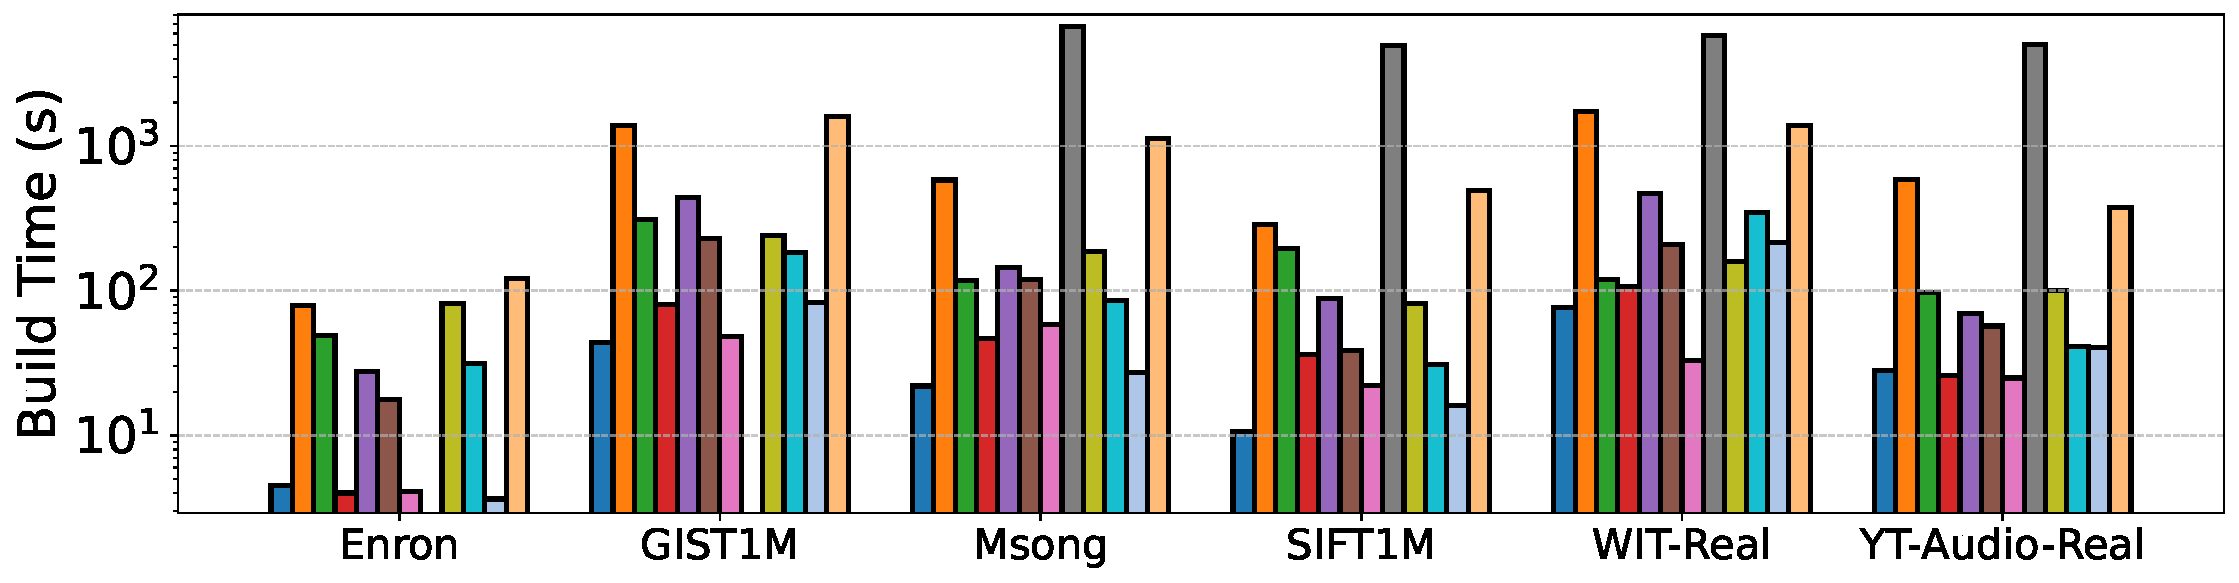
\includegraphics[width=0.95\linewidth]{figures/indexData/exp_7_build_time_comparison_query1.pdf}
			\caption{Construction time}
			\label{fig:build_time_comparison_query1}
		\end{subfigure}
		
		
		
		\begin{subfigure}{\columnwidth}
			\centering
			
			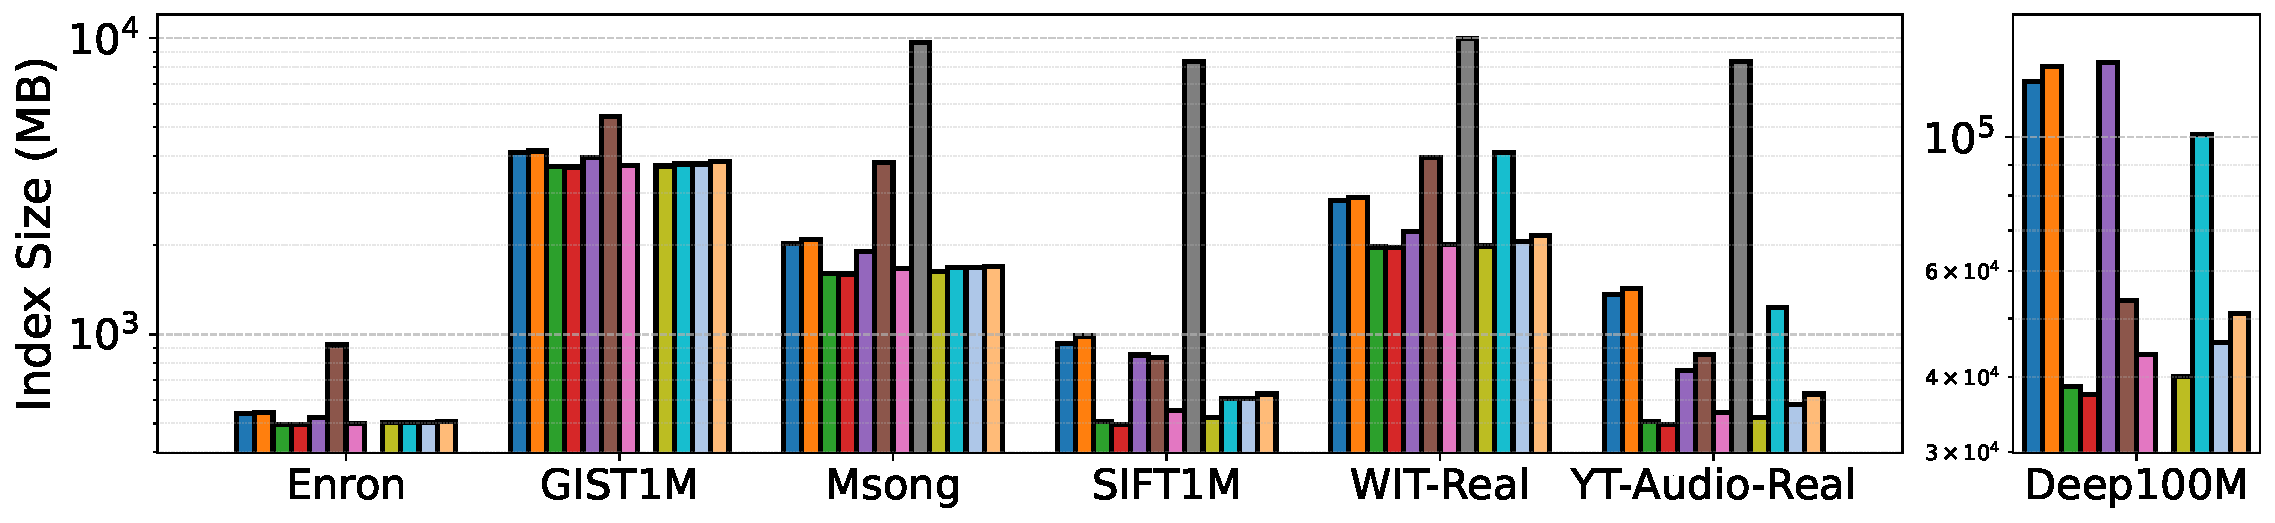
\includegraphics[width=0.95\linewidth]{figures/indexData/exp_7_index_size_mb_comparison_query1.pdf}
			\caption{Index size (including original dataset)}
			\label{fig:index_size_mb_comparison_query1}
		\end{subfigure}
		
		
		
		\begin{subfigure}{\columnwidth}
			\centering
			
			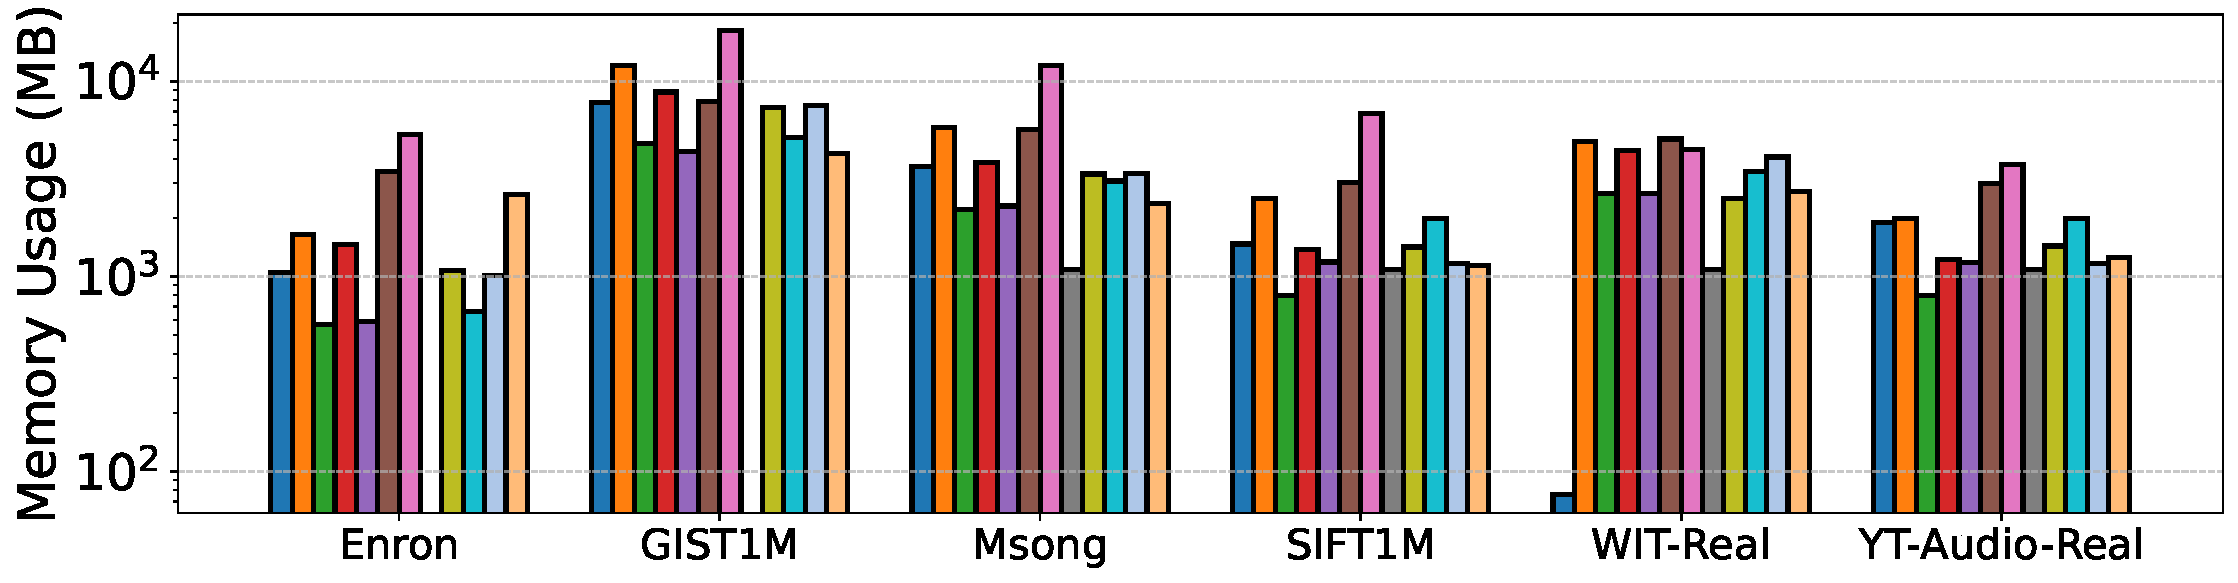
\includegraphics[width=0.95\linewidth]{figures/indexData/exp_7_memory_mb_comparison_query1.pdf}
			\caption{Build peak memory }
			\label{fig:search_memory_mb_comparison}
		\end{subfigure}
		
		\begin{subfigure}{\columnwidth}
			\centering
			
			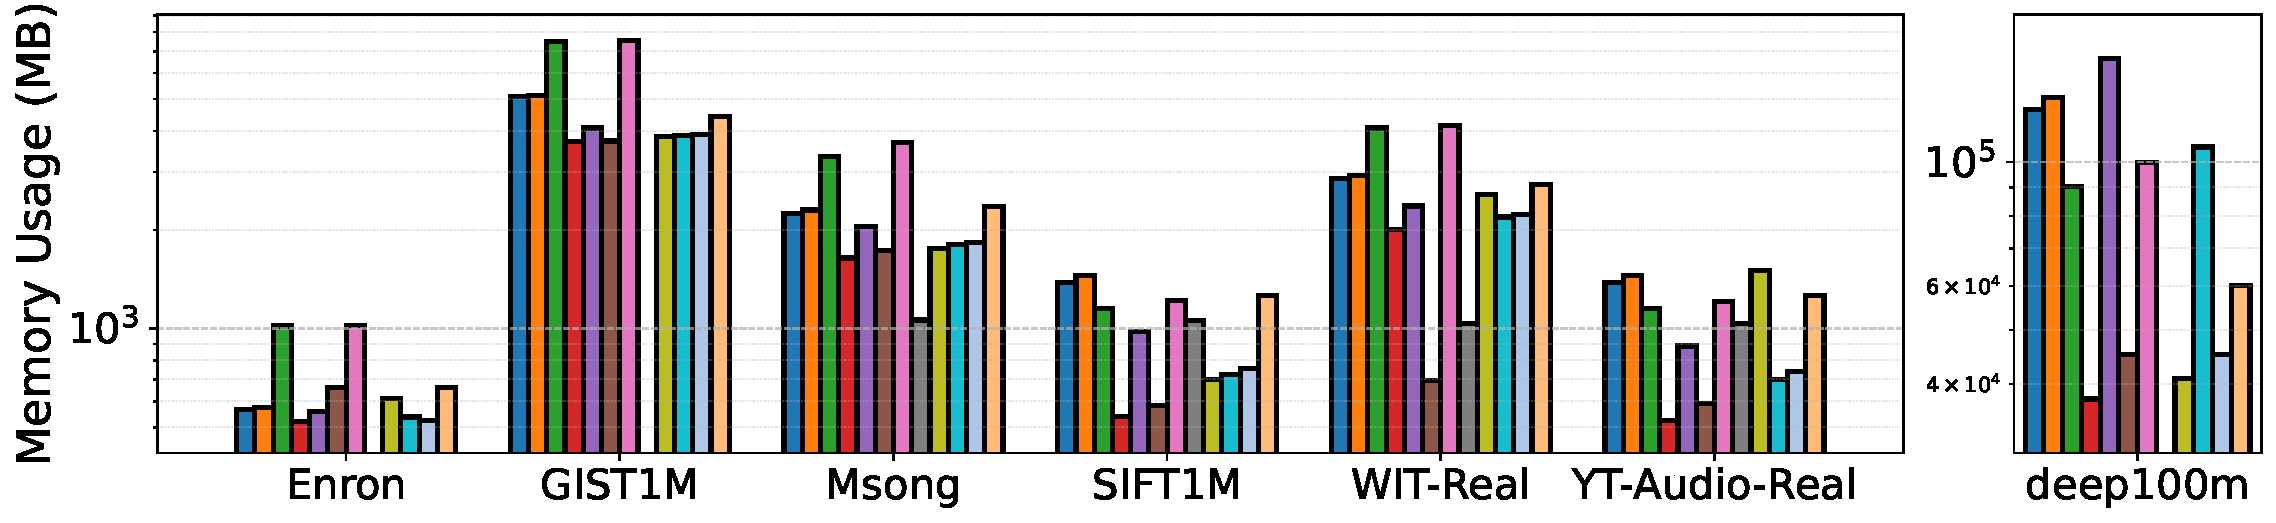
\includegraphics[width=0.95\linewidth]{figures/searchMem/label_memory_comparison.pdf}
			\caption{Search peak memory}
			\label{fig:build_memory_mb_comparison}
		\end{subfigure}
		
		%		\caption{Time and space overhead of attribute filtering index construction}
		\caption{\textcolor{violet}{Time and space overhead}}
		\label{fig:build_index_comparison}
	\end{figure}
	
	
	
	To investigate the performance of different attribute filtering algorithms during index construction, we evaluate 3 key metrics in the single-attribute scenario: index construction time, index size, and peak memory usage. Notably, PASE on GIST1M and Enron is omitted, as it supports only data with dimensionality less than 512. 
	
	\begin{figure*}
		\centering
		
		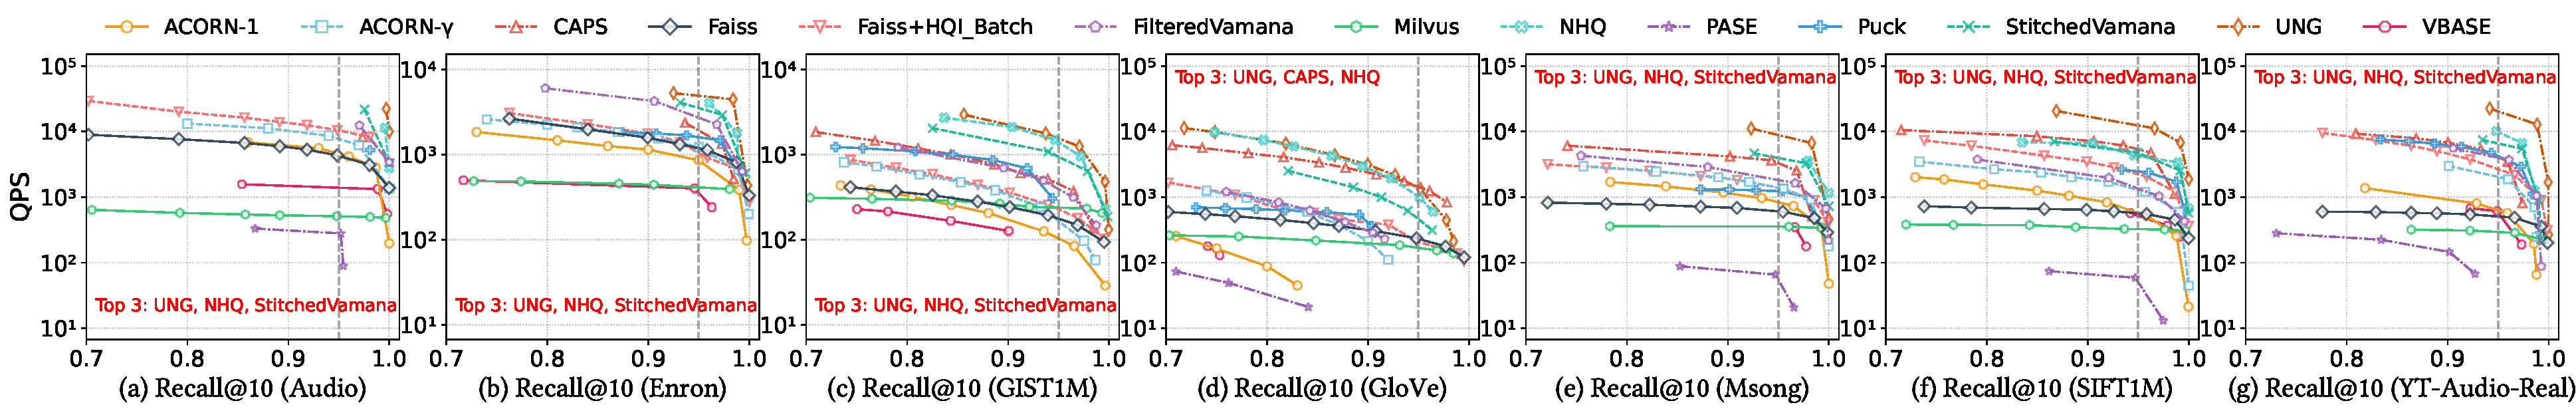
\includegraphics[width=0.95\textwidth]{figures/exp/exp_1_1_SingleLabel_1thread.pdf}
		\caption{Single-Attribute Building and Query (single thread) }
		\label{fig:exp_1_1_SingleLabel_1thread}
	\end{figure*}
	
	\begin{figure*}
		\centering
		
		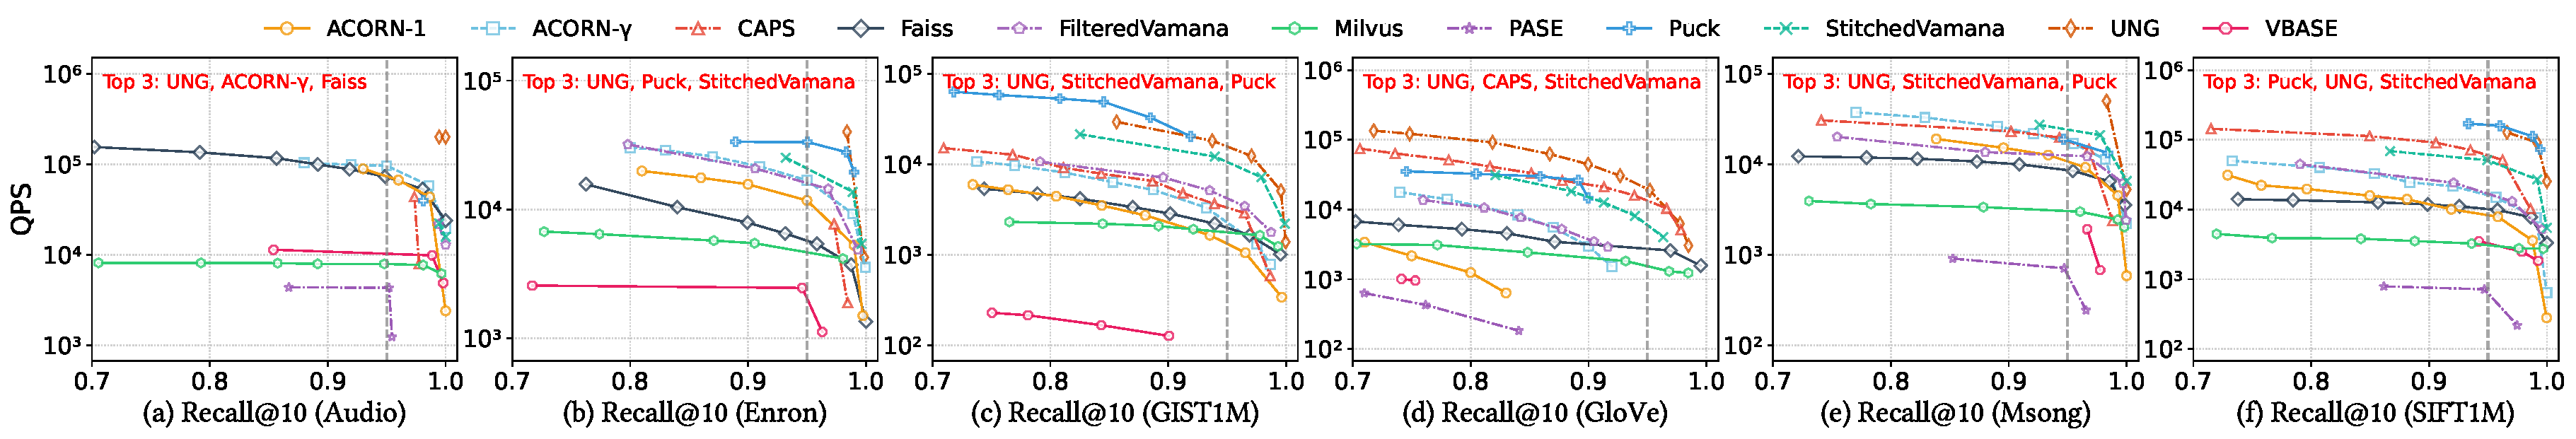
\includegraphics[width=0.95\textwidth]{figures/exp/exp_1_2_SingleLabel_16thread.pdf}
		\caption{Single-Attribute Building and Query (16 threads)}
		\label{fig:exp_1_2_SingleLabel_16thread}
	\end{figure*}
	
	\textit{\textbf{Index construction time.}}
	As shown in Figure~\ref{fig:build_time_comparison_query1}, among the aforementioned 4 datasets, PASE has the longest index construction time due to its single-thread indexing support. Additionally, VBASE also supports only single-thread indexing but achieves better query performance than PASE.
	
	For algorithms supporting 32-thread, index construction time differences are negligible on small-scale datasets (Audio and Enron) due to their limited complexity. On large-scale datasets (SIFT1M, GIST1M, GloVe, and Msong), ACORN-1 achieves the fastest index construction. This efficiency stems from its similarity to the original HNSW construction process and the use of a limited number of candidate neighbors. In contrast, ACORN-$\gamma$ incurs the highest index construction time, as it expands neighbor lists and evaluates a large candidate pool, leading to increased computational overhead.
	
	
	\textit{\textbf{Index size.}}
	%	Traditional graph-based methods often only evaluate the size of the generated graph index and do not include the original data, while the index generated by the IVF-based method includes the original data. In order to unify the comparison standard, 
	%	we include both the index structure generated by the algorithm and the original data when evaluating the index size. 
	%\sout{To ensure a fair comparison with IVF-based algorithms, we include the original dataset in the index size calculation for graph-based indexes.}
	% Traditional graph-based methods often evaluate only the size of the generated index, excluding the original data, whereas IVF-based methods include it. To ensure a consistent comparison, we consider both the index structure and the original data when measuring index size.
	As shown in the Figure~\ref{fig:index_size_mb_comparison_query1}, PASE exhibits significantly larger index sizes across all supported datasets. This overhead stems primarily from its extensive metadata requirements. The index sizes of other methods show moderate variation. Among these, Faiss generates slightly smaller indexes due to its efficient index design.
	
	
	
	\textit{\textbf{Peak memory usage.}}
	As shown in Figure~\ref{fig:memory_mb_comparison_query1}, on small-scale datasets, all methods except NHQ exhibit low memory usage. This is because NHQ adopts the kgraph approach for index construction, which requires loading the entire graph data into memory and maintaining a complete graph structure, leading to relatively high memory overhead. On large-scale datasets, CAPS exhibits slightly lower memory usage compared to other algorithms. \textcolor{orange}{The reason is that CAPS avoids redundant storage and graph structure overhead through hierarchical partitioning and AFT, and achieves a compact, sparse and controllable index. }Due to their special characteristics, databases are not included in the peak memory usage testing during index construction.
	
	
	
	\subsubsection{Performance Evaluation}
	
	
	%4.2.2
	
	
	We next evaluate the query performance of AF-ANN search methods, focusing on 3 main scenarios.
	
	\textit{\textbf{Single-Attribute Building and Single-Attribute Query.}}
	In this scenario, we construct the index using an attribute and apply filtering conditions on the same attribute.
	
	
	\textit{Single-Thread Search.}  
	As shown in Figure~\ref{fig:exp_1_1_SingleLabel_1thread}, under full-recall conditions (recall = 1), search often requires traversing larger candidate sets or deeper graph paths, leading to increased computational cost and a sharp QPS drop for most methods. Despite this, UNG maintains high QPS due to its LNG structure, which eliminates unnecessary online filtering of irrelevant attributes, thereby improving query efficiency. But, UNG slightly underperforms on high-LID datasets such as GloVe. In contrast, CAPS performs better on high-LID datasets but is more sensitive to dataset characteristics. CAPS leverages multi-level spatial partitioning and attribute filtering to efficiently explore sparse spaces, whereas UNG relies on structured attribute organization, which limits its adaptability to sparse high-dimensional distributions.
	
	NHQ, StitchedVamana, and FilteredVamana show similar and stable performance across all datasets. This indicates that joint filtering and search strategies can achieve consistent effectiveness under high-recall requirements. As observed in Figure~\ref{fig:exp_1_1_SingleLabel_1thread}, StitchedVamana outperforms FilteredVamana in query efficiency. The difference arises from their pruning strategies: StitchedVamana applies pruning after merging graphs, allowing nodes to accumulate a richer candidate set; while FilteredVamana applies early pruning, potentially eliminating useful candidates prematurely.
	
	Among all methods, vector database systems (PASE, VBASE, Milvus) perform the worst. These systems target general-purpose scenarios but incur communication latency from network I/O and experience high query processing overhead due to complex query parsing. Additionally, we observe that Faiss+HQI\_Batch outperforms original Faiss, indicating that batch querying via HQI can effectively enhance query performance.
	
	\textit{Multi-Thread Search.}
	As shown in Figure~\ref{fig:exp_1_2_SingleLabel_16thread}, UNG continues to achieve the best performance. 
	%Puck performs well on large-scale datasets, but its performance degrades on small datasets. Puck is tailored for large-scale scenarios, and optimizations such as two-level inverted indexing and hierarchical quantization introduce unnecessary overhead on small datasets. 
	Puck performs well on large datasets but degrades on smaller ones due to overhead from optimizations like two-level inverted indexing and hierarchical quantization. CAPS maintains a relatively high throughput under multi-threads but exhibits limited adaptability to different datasets. The vector distribution of the dataset affects the construction of its partitioned index.
	 ACORN performs poorly overall, primarily due to the sensitivity of its hyperparameter $\gamma$ to attribute selectivity. Without careful tuning based on dataset characteristics, it is challenging to construct an effective index.
	
	\textit{\textbf{Multi-Attribute Building and Single-Attribute Query.}}
	In this scenario, the index is constructed using 8 attributes but applies filtering condition on only 1 attribute during the query.
	
	Faiss offers an ID filtering mechanism, it operates solely during query execution and does not influence index building. ACORN is   designed for single-attribute indexing. In database systems (VBASE, PASE, Milvus), 
	%\sout{when the system builds both B+ tree and vector indexes, queries typically utilize only the B+ tree.} 
	attributes do not participate in index construction.
	Hence, they are excluded from this comparison.
	
	\begin{figure}[t]
		\centering
		
		% 上面的图例,居中并可通过 hspace 调整左右位置
		\hspace*{15pt} % 可调整的参数,负值左移,正值右移,例如 -20pt 或 20pt
		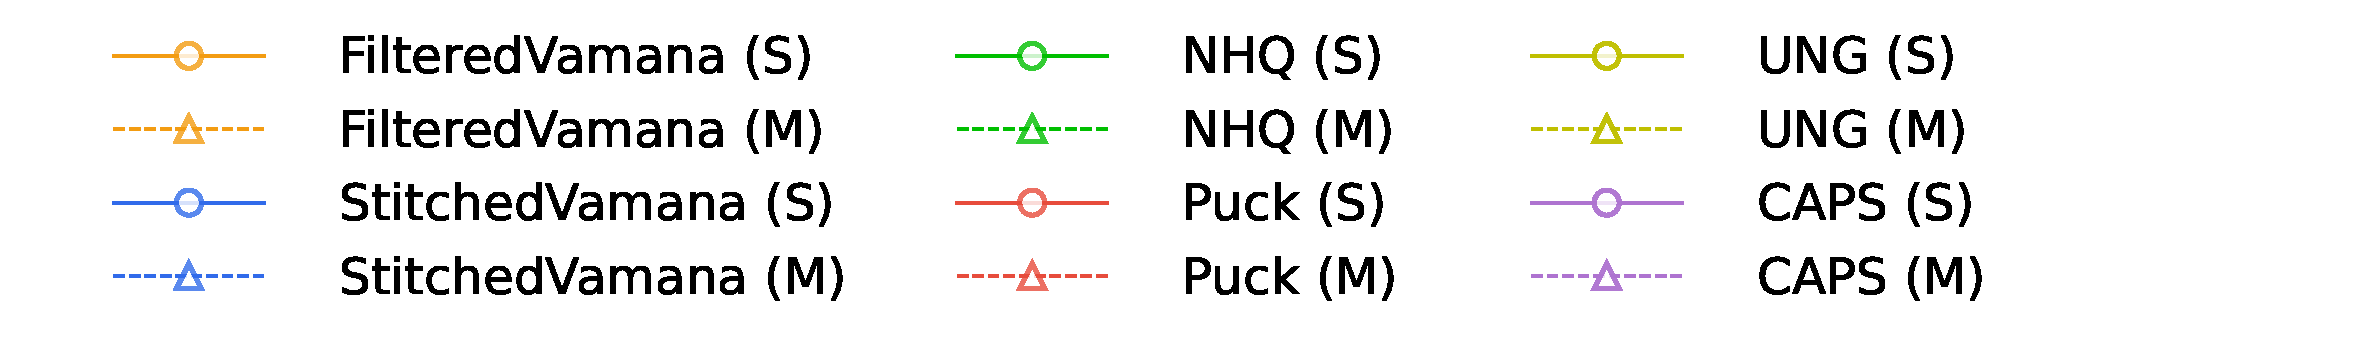
\includegraphics[width=0.85\columnwidth]{figures/exp/exp_2_legend.pdf} % 图例图片路径
		
		
		% 下面的子图,居中显示
		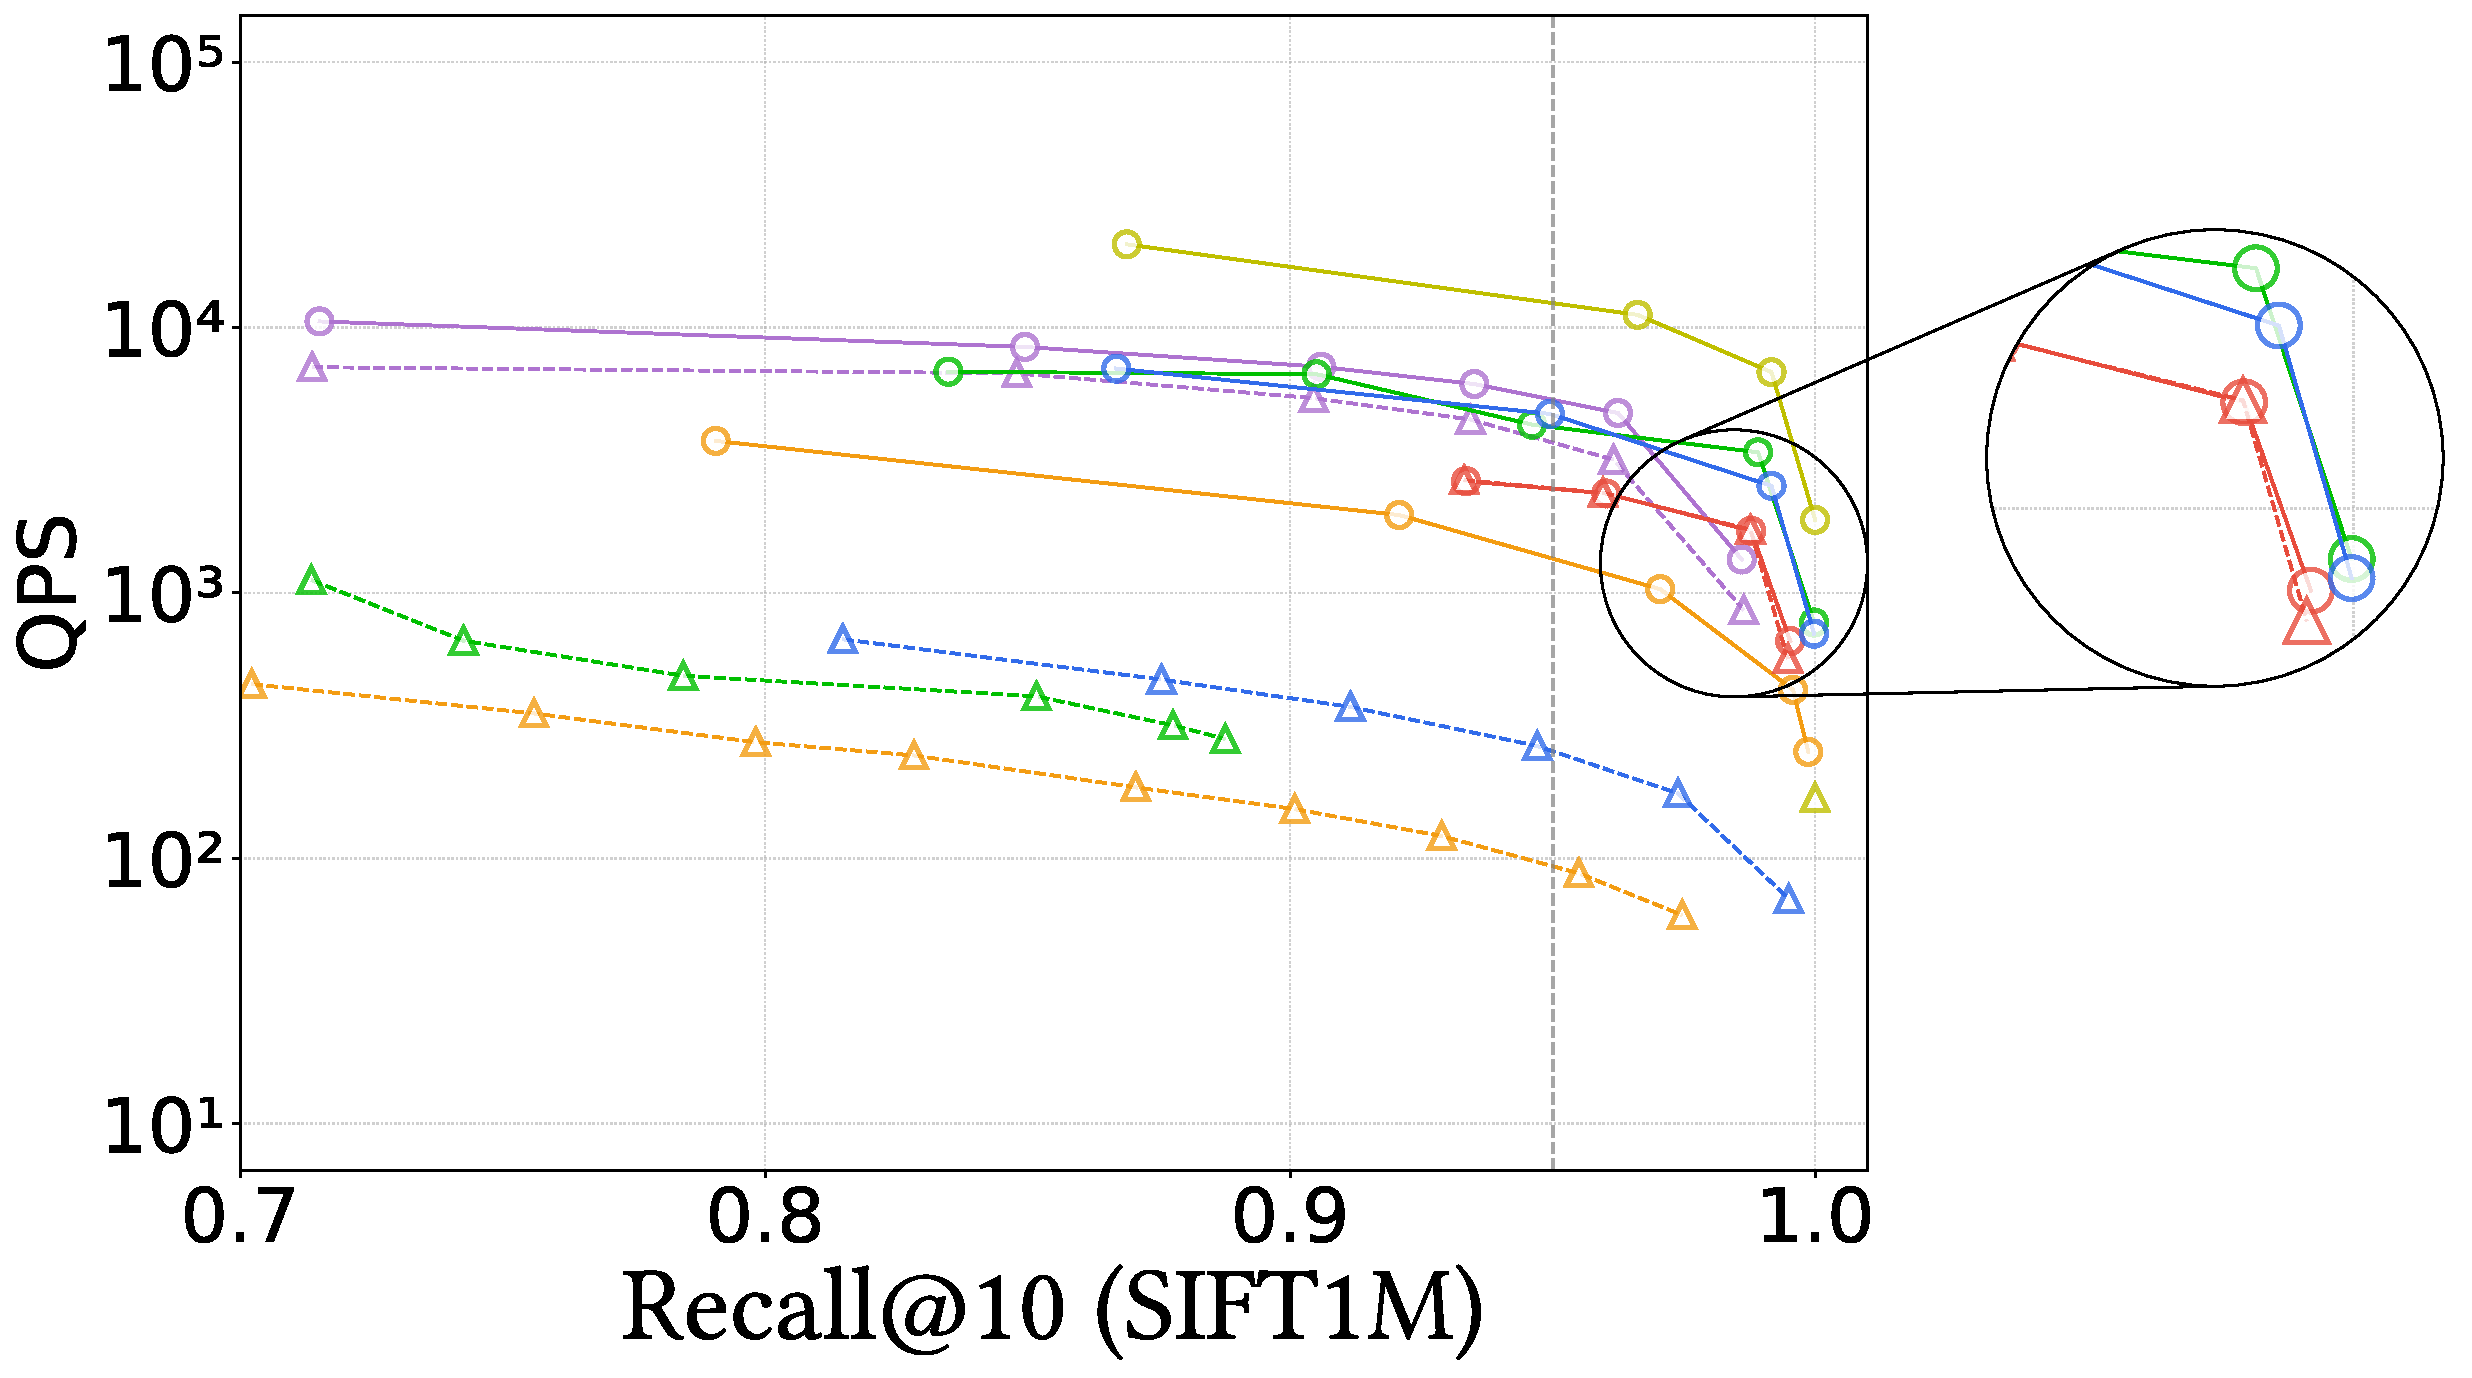
\includegraphics[width=0.7\columnwidth]{figures/exp/exp_2_1.pdf}
		\caption{Effect of Multi-Attribute Index Construction on Single Query Performance. ($S$ denotes single-attribute index construction and single-attribute query; $M$ denotes multi-attribute index construction and single-attribute query)}
		\label{fig:exp_2_1}
		
	\end{figure}
	
	\textit{Effect of Multi-Attribute Building on Algorithm Performance (M vs. S).}
	As shown in Figure \ref{fig:exp_2_1}, Puck demonstrates nearly no performance degradation.  CAPS shows a slight performance decline due to the increased query overhead caused by excessive attribute-based grouping. In contrast, the performance of StitchedVamana, FilteredVamana, NHQ, and UNG drops significantly, with the following reasons: 1) FilteredVamana increases the complexity introduced by retaining attribute during index construction. 2) The complexity of StitchedVamana increases because data points may duplicate across multiple subgraphs. 3) The fusion distance of NHQ exhibits sensitivity to the number of attributes, which degrades its effectiveness. 4) UNG has poor performance because large number of entry points that need to be traversed. It is difficult for a graph with multiple entries to have good connectivity, degenerating into a situation closer to inverted retrieval, and the effect may be greatly impaired.
	
	
	
	\textit{Performance of Algorithms under Multi-Attribute Building (M vs. M).}  
	As shown in Figure \ref{fig:exp_2_1}, IVF-based methods (Puck and CAPS) significantly outperform graph-based methods. The reason for Puck's superior performance is that it filters out irrelevant results during the retrieval process rather than searching for more candidates. CAPS performs as well as Puck. In contrast, FilteredVamana performs the worst because its multi-attribute indexing forces neighbor selection to cover multiple attributes, reducing the efficiency of single-attribute queries. This results in excessive traversal of irrelevant nodes, making it slower than other methods.
	
	
	\begin{figure*}
		\centering
		
		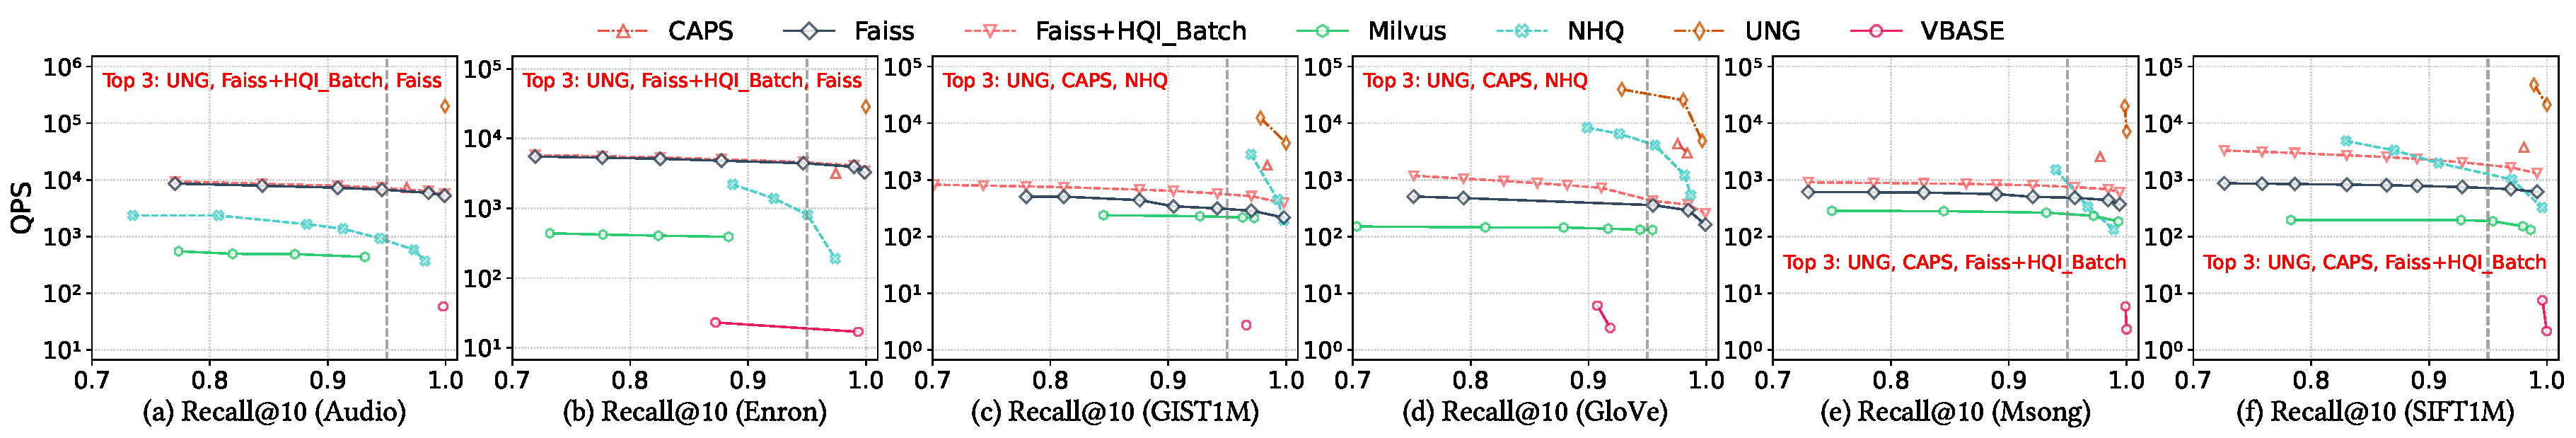
\includegraphics[width=0.95\textwidth]{figures/exp/exp_4_1_MultiLabel_1thread.pdf}
		\caption{Multi-attribute build and query (single thread)}
		\label{fig:exp_4_1_MultiLabel_1thread}
	\end{figure*}
	
	\begin{figure*}
		\centering
		
		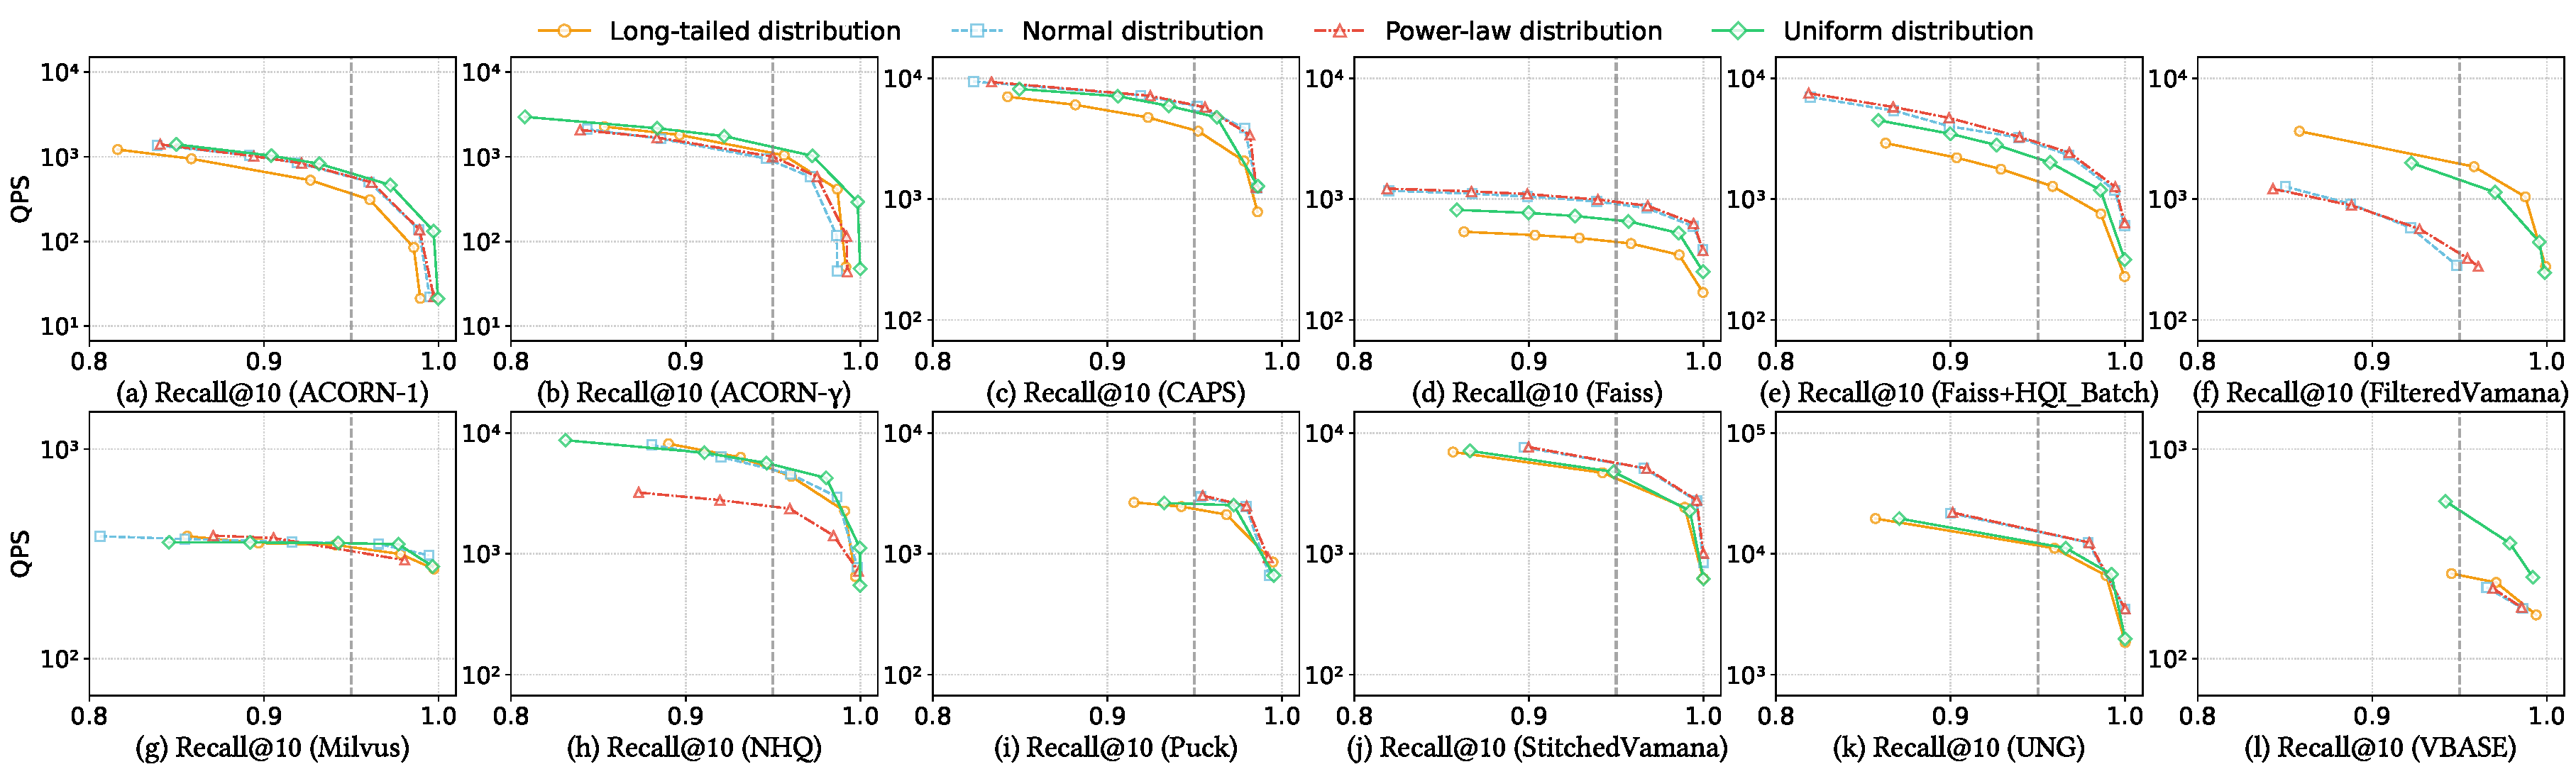
\includegraphics[width=0.95\textwidth]{figures/exp/exp_3_1.pdf}
		\caption{Effect of attribute distribution on query performance (single thread)}
		\label{fig:exp_3_1}
	\end{figure*}
	
	
	
	
	
	\textit{\textbf{Multi-Attribute Building and Multi-Attribute Query.}}  
	Compared to single-attribute filtering, multi-attribute joint filtering better reflects real-world scenarios. To evaluate algorithm performance under this setting, we construct the index using 3 uniformly distributed attributes and apply filtering on all 3 attributes simultaneously during queries.
	%	\textcolor{red}{As Filtered-DiskANN does not support the AND rule used in our multi-attribute queries, it is excluded.}
	%	Compared to single-attribute filtering, multi-attribute joint filtering better reflects real-world application scenarios. To evaluate algorithm performance under such scenario, we construct the index using 3 uniformly distributed attributes and apply filtering conditions on all 3 attributes simultaneously during the query process.
	
	As shown in Figure~\ref{fig:exp_4_1_MultiLabel_1thread}, UNG achieves the best performance across all datasets. For IVF-based methods not specifically optimized for hybrid queries (Faiss\_IVF and Milvus), their QPS remains relatively stable as recall varies. Milvus, as a general-purpose system, exhibits comparatively poor performance. 
	

		The IVF-based algorithm Faiss---especially when combined with HQI\_Batch---achieves moderate performance. It naturally supports pre-filtering and remains unaffected by the increasing number of attributes. In fact, filtering can reduce the effective candidate set, thereby improving search efficiency. In contrast, the IVF-based algorithm CAPS, which is optimized for hybrid queries, employs a multi-level partitioning strategy that introduces additional overhead. This overhead negatively impacts performance on small datasets. However, on large datasets, the overhead is amortized, and the advantages of attribute-aware partitioning become evident, making CAPS the second-best performer after UNG.
	
	
	%	In contrast, Faiss—especially when combined with HQI\_Batch—achieves medium-level performance. Its original IVF implementation naturally supports pre-filtering and does not suffer from the complexity introduced by an increased number of attributes. In fact, filtering can reduce the effective candidate set, improving efficiency.
	%	As shown in Figure~\ref{fig:exp_4_1_MultiLabel_1thread}, UNG achieves the best performance across all datasets. For IVF-based methods that are not specifically optimized for hybrid query scenarios (Faiss\_IVF and Milvus), their QPS remains relatively stable as the recall varies. Milvus, being a general-purpose system, exhibits comparatively poor performance. In contrast, Faiss—especially when combined with HQI\_Batch—achieves medium-level performance. Its original IVF implementation naturally supports pre-filtering and does not suffer from the complexity introduced by an increased number of attributes. In fact, filtering can reduce the effective candidate set, improving efficiency.
	
	%	The IVF-based algorithm CAPS, optimized for hybrid queries, employs a multi-level partitioning strategy that introduces additional overhead. This overhead negatively impacts performance on small datasets. However, on large datasets, the overhead is amortized, and the benefits of attribute-aware partitioning become evident, making CAPS the second-best performer after UNG.
	
	%	NHQ exhibits mediocre performance overall and performs particularly poorly on small datasets. It relies on fusion distance calculations. The fusion distance computation is highly sensitive to the number of attributes involved, thus impacting both efficiency and accuracy under multi-attribute filtering.
	NHQ performs moderately overall but poorly on small datasets. Its reliance on fusion distance computations makes it highly sensitive to the number of attributes, impacting both efficiency and accuracy under multi-attribute filtering.
	
	
	
	
	\subsubsection{Robustness}In the following, we evaluate the robustness of these algorithms.
	
	\textit{\textbf{Attribute Distribution.}} To evaluate performance across different attribute distributions, we generate base and query attribute sets with 4 representative distributions—long-tailed, normal, power-law, and uniform—across the 6 datasets described in Section~4.1.1. We evaluate all algorithms under these distributions on each dataset. The performance differences observed for the same algorithm across different datasets are relatively minor. Thus, due to space constraints, we present only the results on SIFT1M.
	
	As illustrated in Figure~\ref{fig:exp_3_1}, the evaluated algorithms exhibit varying degrees of sensitivity to attribute distribution shifts. \textcolor{blue}{The closer the four curves (corresponding to the four distributions) in the figure approach each other, the less the algorithm is affected by attribute distributions. Conversely, the farther they diverge, the more significant the impact of attribute distributions on the algorithm becomes.} Specifically, ACORN, Milvus, Puck, CAPS, StitchedVamana, and UNG demonstrate strong robustness to such shifts. In contrast, Faiss, FilteredVamana, NHQ, VBASE, and PASE show notable sensitivity.
	
	Among all algorithms, ACORN-\(\gamma\) shows the highest robustness. During index construction, attribute is mainly used for pruning in the lowest layer graph, while the upper-layer hierarchical navigation graphs remain largely unaffected. As a result, changes in attribute distribution have a limited impact on overall performance.
	
	In contrast, VBASE exhibits the weakest robustness. As a post-filtering system, it performs significantly better under uniform distributions but degrades under long-tailed, normal, and power-law distributions. This degradation stems from the low selectivity of certain attributes in the last 3 distributions, which increases unnecessary distance computations, thus reducing overall efficiency.
	
	\begin{figure}
		\centering
		\setlength{\abovecaptionskip}{0.1cm}
		\setlength{\belowcaptionskip}{-0.1cm}
		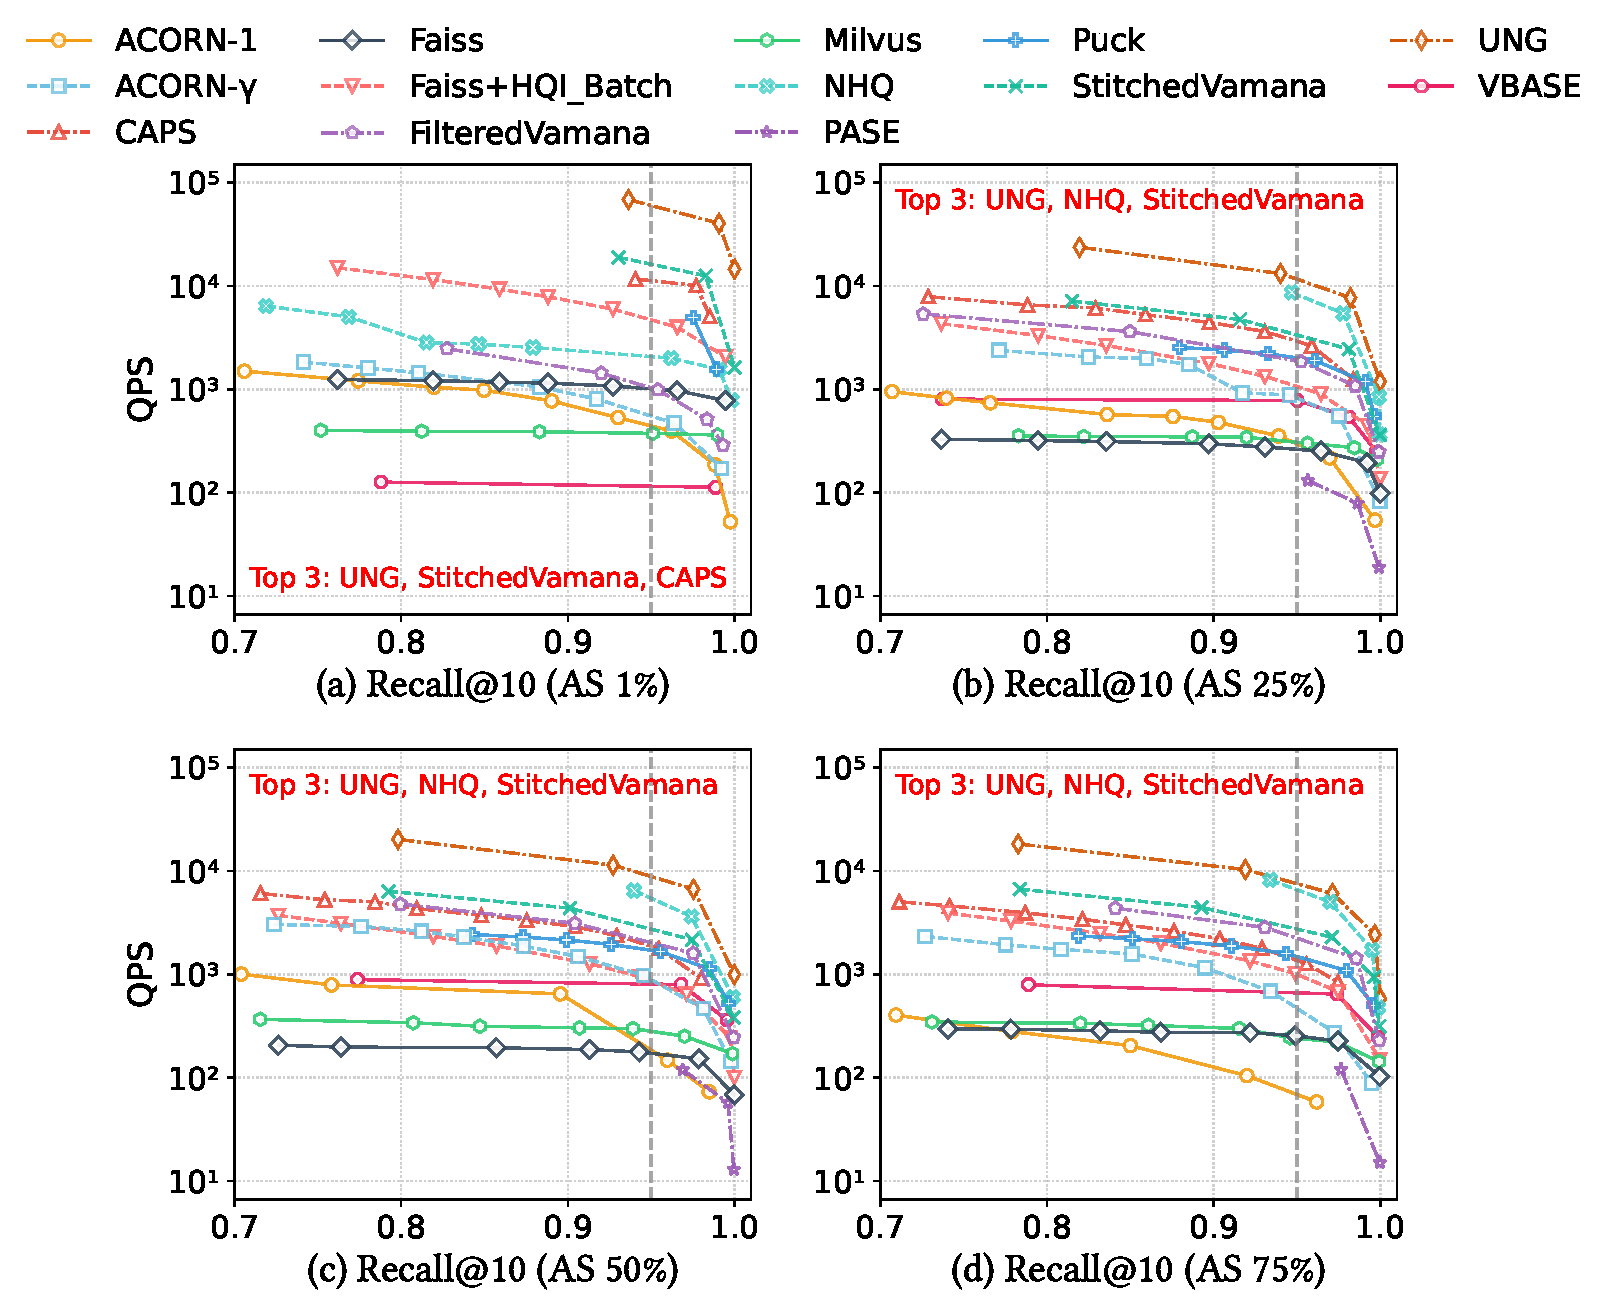
\includegraphics[width=0.95\columnwidth]{figures/exp/exp_5_1_1_SingleLabel_1thread.pdf}
		\caption{Effect of Single-Attribute Selectivity on Query}
		\label{fig:exp_5_1_1_SingleLabel_1thread}
	\end{figure}
	
	
	\textit{\textbf{Single-Attribute Selectivity.}}
	In hybrid queries, varying attribute selectivity (AS) can significantly impact computational cost and query efficiency, as the algorithm must efficiently identify data points matching specific attributes within large datasets. AS is defined as the proportion of data points sharing a given attribute value. For example, AS of 1\% indicates that only 1\% of the dataset meets the given attribute. 
	
	To investigate this effect, we evaluate 4 AS settings (1\%, 25\%, 50\%, and 75\%) on the SIFT1M dataset using single-thread execution. We compare the query performance of attribute filtering algorithms across these settings, as shown in Figure~\ref{fig:exp_5_1_1_SingleLabel_1thread}.
	
	Experimental results show that UNG achieves the best performance across all AS settings, especially at extremely low AS (1\%). 
	This advantage stems from its pre-filtering strategy. Pre-filtering strategy significantly reduces the ANN search space by narrowing down candidates prior to vector computation. In contrast, VBASE performs the worst at 1\% AS due to its post-filtering strategy. Post-filtering strategy first retrieves a large number of candidates and then applies filtering, incurring substantial computational overhead.
	
	
	
	
	\begin{figure*}
		\centering
		
		% 第一行:单独一张大图
		\begin{subfigure}{\textwidth}
			\centering
			
			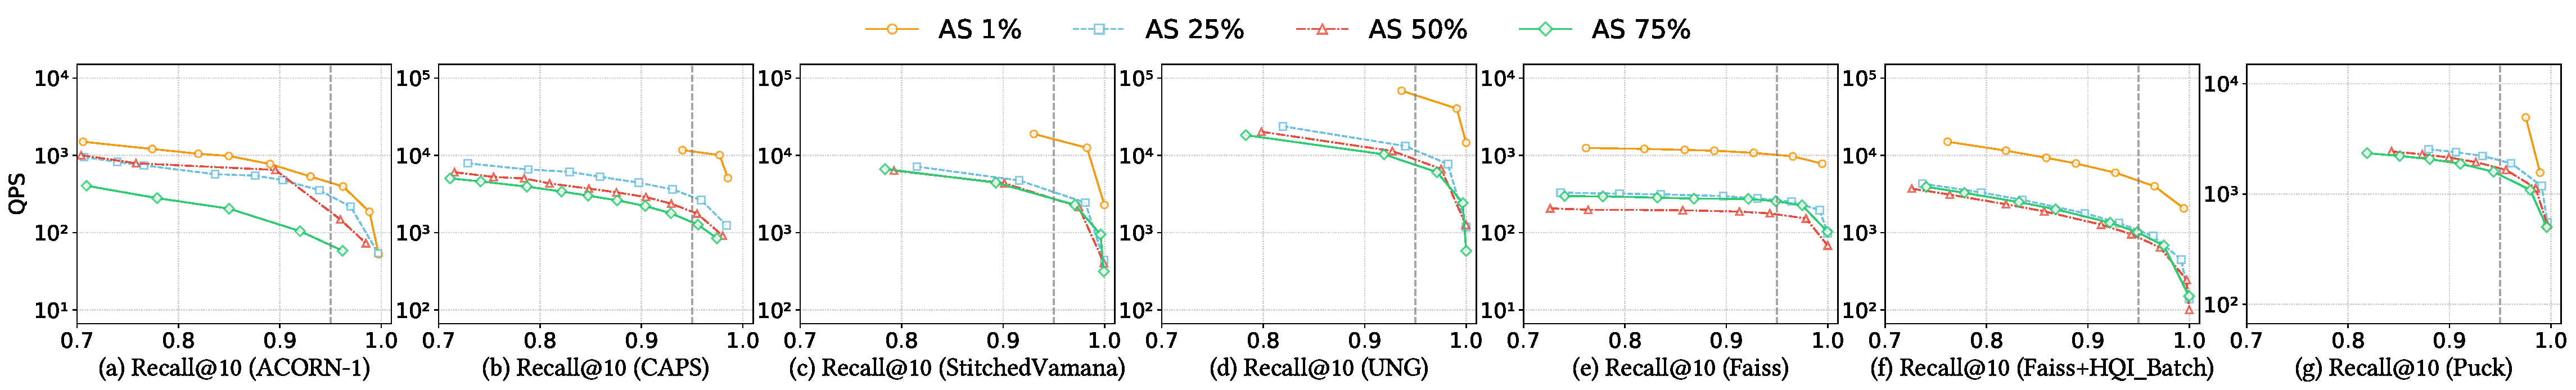
\includegraphics[width=0.95\textwidth]{figures/exp/exp_5_2_1.pdf}
			\caption{Algorithms optimized for low AS.}
			\label{fig:exp_5_2_1}
		\end{subfigure}
		
		\vfill % 增加垂直间距
		
		% 第二行:两张子图,左侧宽度是右侧的两倍
		\begin{subfigure}{0.64\textwidth} % 2/3 宽度
			\centering
			
			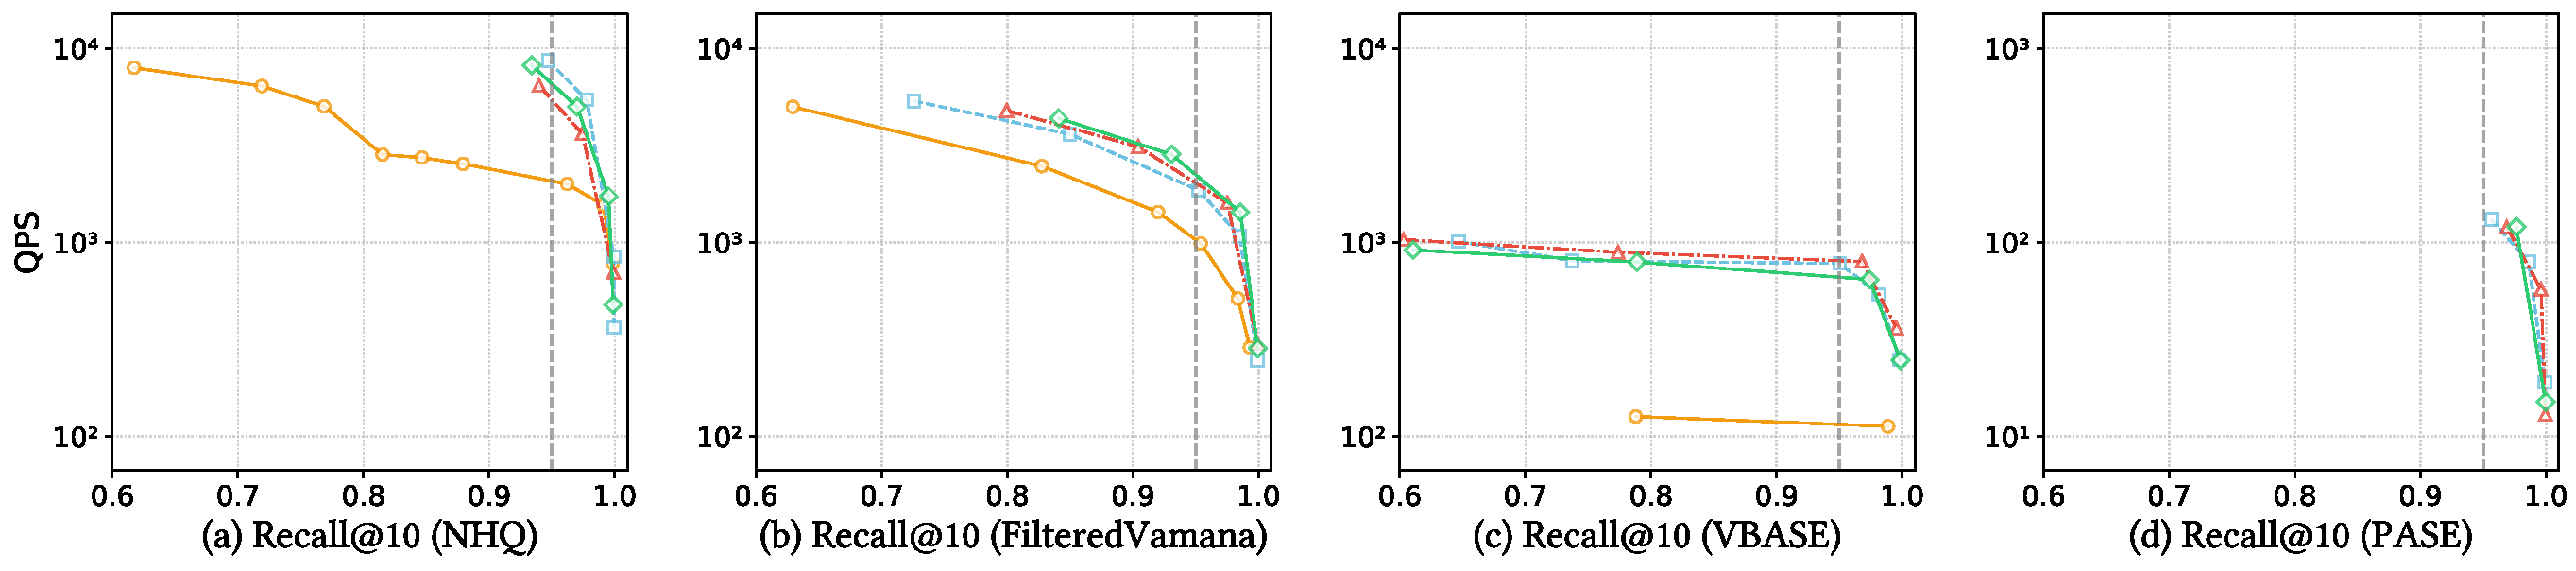
\includegraphics[width=0.92\textwidth]{figures/exp/exp_5_2_2.pdf}
			\caption{Algorithms optimized for high AS.}
			\label{fig:exp_5_2_2}
		\end{subfigure}
		\hspace{1mm} % 增加水平间距
		\begin{subfigure}{0.32\textwidth} % 1/3 宽度
			\centering
			
			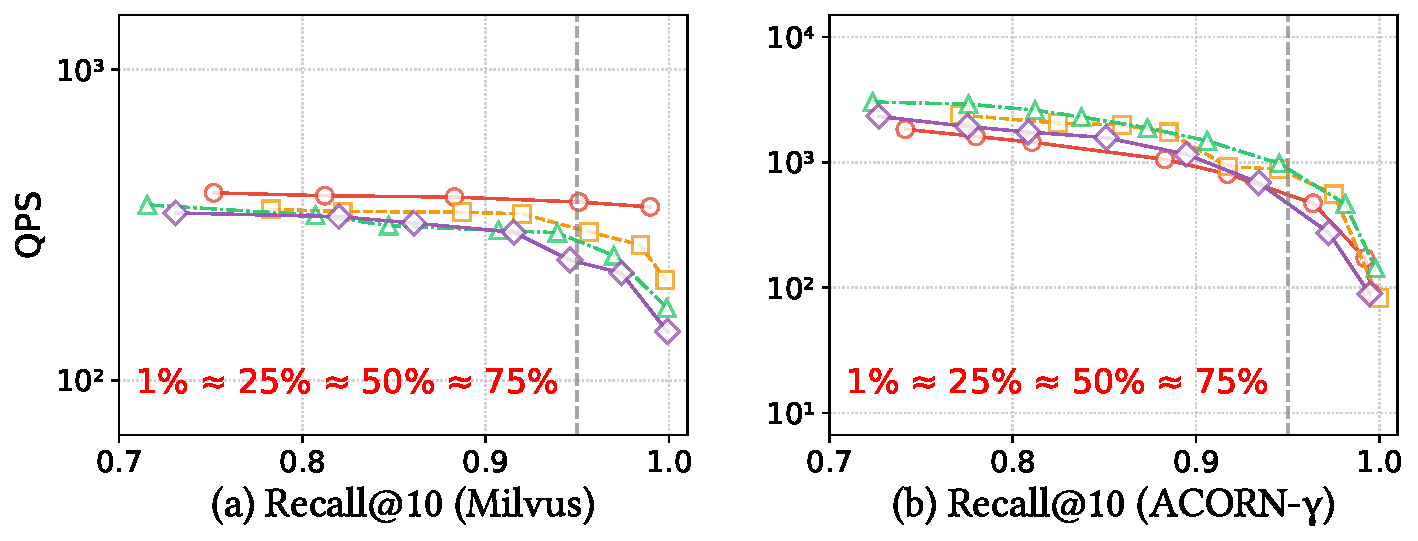
\includegraphics[width=0.92\textwidth]{figures/exp/exp_5_2_3.pdf}
			\caption{Algorithms insensitive to AS.}
			\label{fig:exp_5_2_3}
		\end{subfigure}
		
		
		\caption{Different AS under the same algorithm}
		\label{fig:exp_5_2_combined}
	\end{figure*}
	
	
	Based on the query performance trends of different algorithms under varying AS, we categorize the algorithms into 3 groups:
	
	(1) \textit{Algorithms optimized for low AS.}  
	This group includes ACORN-1, Faiss+HQI\_Batch, StitchedVamana, UNG, Faiss, Puck, and CAPS, as illustrated in Figure~\ref{fig:exp_5_2_1}.
	
	ACORN-1 performs well in low AS because fewer nodes share the same attribute. This increases the average degree of retained nodes and improves graph connectivity. CAPS efficiently skips irrelevant subpartitions, reducing computational overhead. However, as AS increases, it must process more subpartitions and handle a larger dataset. StitchedVamana optimizes local adjacency using independent subgraphs, enabling fast localization at low AS. However, at higher AS, it requires broader global exploration. UNG, Faiss, and Puck all use pre-filtering strategies to shrink the search space in low AS, leading to better performance.
	
	Interestingly, Faiss and Faiss+HQI\_Batch perform worst at the 50\% AS instead of 75\%.
	%, which might seem unexpected. 
	This happens because, when AS decreases from 75\% to 50\%, fewer data points are filtered out. As a result, more clusters must be searched, increasing computational cost.
	
	\par
	(2) \textit{Algorithms optimized for high AS.}  
	This group includes NHQ, FilteredVamana, VBASE, and PASE, as shown in Figure~\ref{fig:exp_5_2_2}.
	
	At low AS, NHQ struggles to locate relevant regions efficiently, leading to excessive computations on non-matching nodes. FilteredVamana also performs poorly in these scenarios. Its dynamic pruning strategy makes it difficult to balance vector distance and attribute relevance, resulting in overly restricted search paths.
	VBASE relies on post-filtering, which increases computational overhead at low AS. PASE performs poorly at extremely low AS (e.g., 1\%), with recall dropping below 0.2. Its fixed candidate set may not contain enough valid results after filtering, leading to incomplete top-$k$ results and significantly reducing recall.
	
	\par
	(3) \textit{Algorithms insensitive to AS.}  
	This group includes Milvus and ACORN-\(\gamma\), as illustrated in Figure~\ref{fig:exp_5_2_3}.
	
	Milvus is mainly limited by system-level communication overhead, such as API latency. As a result, its query performance remains largely unaffected by AS variations. ACORN-\(\gamma\) maintains stable performance across different AS settings by using a higher index construction parameter $\gamma$. This ensures a relatively stable average node degree, even after attribute pruning, minimizing the impact of AS changes on query efficiency.
	
	\begin{figure*}
		\centering
		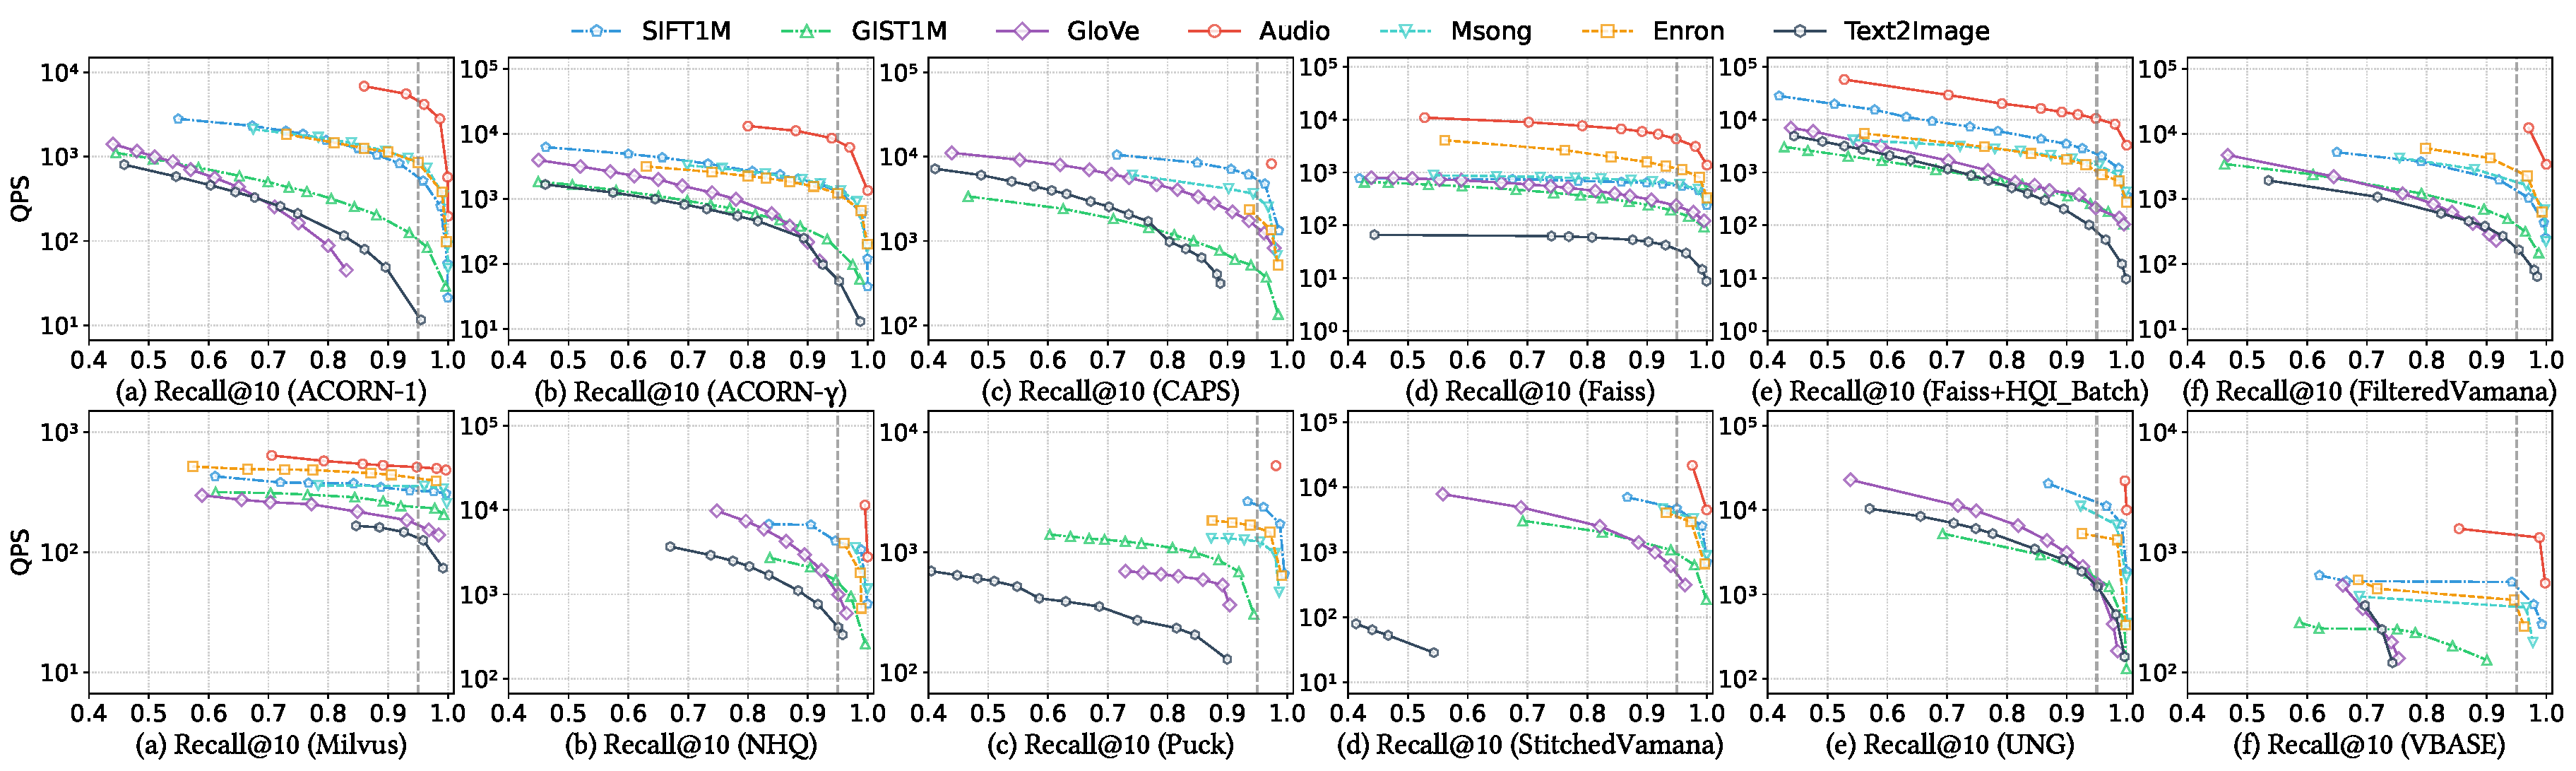
\includegraphics[width=0.95\textwidth]{figures/exp/exp_6_1.pdf}
		\caption{Effect of dataset on Query}
		\label{fig:exp_6_1}
	\end{figure*}
	
	%4.2.7
	
	% \begin{table}[t]
		% 	\centering
		% 	\setlength{\abovecaptionskip}{0.05cm}
		% 	\caption{Time and space overhead of range filtering index construction}
		
		% 	\label{tab:Range Filtered}
		% 	\resizebox{\columnwidth}{!}{
			% 		\begin{tabular}{l l c c c c c }
				% 			\toprule
				% 			\textbf{Dataset} & \textbf{Metric} & \textbf{DSG} & \textbf{iRange} & \textbf{SeRF} & \textbf{UNIFY} & \textbf{WinFilter} \\
				% 			\midrule
				% 			\multirow{3}{*}{DEEP} 
				% 			& Index time(s)  & 4156 & 1128 & \textbf{189.89} & 7510 & 32843 \\
				% 			& Index size(GB)  &  4.6 & 0.92 & \textbf{0.80} & 1.43 & 2.41  \\
				% 			& Peak memory(GB) &  7.78 & 3.54 & \textbf{1.38} & 2.61 & 7.08   \\
				% 			% \cmidrule{1-7}
				% 			\midrule
				% 			\multirow{3}{*}{YT-Audio} 
				% 			& Index time(s)   & 15314 & 1039 & \textbf{187.20} & 5905 & 30904    \\
				% 			& Index size(GB)    & 4.3 & \textbf{0.7} & 1.04 & 1.55 & 1.32  \\
				% 			& Peak memory(GB)   & 7.5 & 3.16 & \textbf{1.57} & 2.97 & 6.95  \\
				% 			\midrule
				% 			\multirow{3}{*}{WIT} 
				% 			& Index time(s)  & 29492 & 7068 & \textbf{828.12} & 28759 & 94909\\
				% 			& Index size(GB) &  4.2 & \textbf{1.5 }& 15.34 & 8.71 & 1.59  \\
				% 			& Peak memory(GB)  & 21.7 & \textbf{12.32} & 15.87 & 24.38 & 15.29\\
				% 			% \cmidrule{1-7}
				% 			\bottomrule
				% 		\end{tabular}
			% 	}
		% \end{table}
	
	\textit{\textbf{Different Datasets.}}  
	To evaluate the performance of various methods across different datasets, we conduct experiments on 7 datasets, including one dataset Text2Image for OOD queries. Our analysis focuses on performance variations concerning dataset size, LID, and vector dimensionality.
	
	As shown in Figure~\ref{fig:exp_6_1}, all methods achieve their highest QPS and recall on Audio dataset. Because Audio has small scale, low dimensionality, and low LID. In contrast, all methods exhibit the lowest QPS and recall on the GIST1M and GloVe dataset besides the OOD dataset Text2Image. Because these two datasets have the largest scale and highest LID.
	
	SIFT1M and Msong are similar datasets, with the key difference being that SIFT1M has lower dimensionality. The 4 algorithms (ACORN, Faiss, PASE, and NHQ) perform similarly on these two datasets, suggesting strong robustness to high dimensional datasets. In contrast, the remaining algorithms exhibit degraded performance on Msong, revealing a lack of adaptability to high dimensional datasets.
	
	Most algorithms struggle to achieve high recall on GloVe, because it has the highest LID. Compare to other algorithms, the 4 algorithms (UNG, Faiss, CAPS, and Milvus) manage to maintain relatively high recall, demonstrating better adaptability to complex datasets. Notably, although vanilla Faiss performs worse on SIFT1M compared to Enron dataset, Faiss+HQI\_Batch outperforms on SIFT1M. Because batch optimization in HQI reduces query overhead and increases throughput.
	
	Most algorithms exhibit the worst performance on the OOD dataset Text2Image. However, ACORN, UNG, and FilteredVamana show relatively stable performance on Text2Image. Their performance drops less compared to in-distribution (ID) datasets such as GIST1M and GloVe, indicating better adaptability to OOD queries.
	
	\textit{\textbf{Multimodel, 85 and Deep100M.}} \textcolor{red}{The fig is Figure \ref{fig:TrinityExtension——Attribution}}
	
	\begin{figure}[t]
		\centering
		
		
		\hspace*{5pt}
		% 放大的图例(占满单栏)
		
\includegraphics[width=0.98\columnwidth]{figures/exp/attribute_legend.pdf}
		
		%\vspace{0.1cm}
		\begin{subfigure}[t]{0.332\columnwidth}
			\centering
			\captionsetup{font=small}
			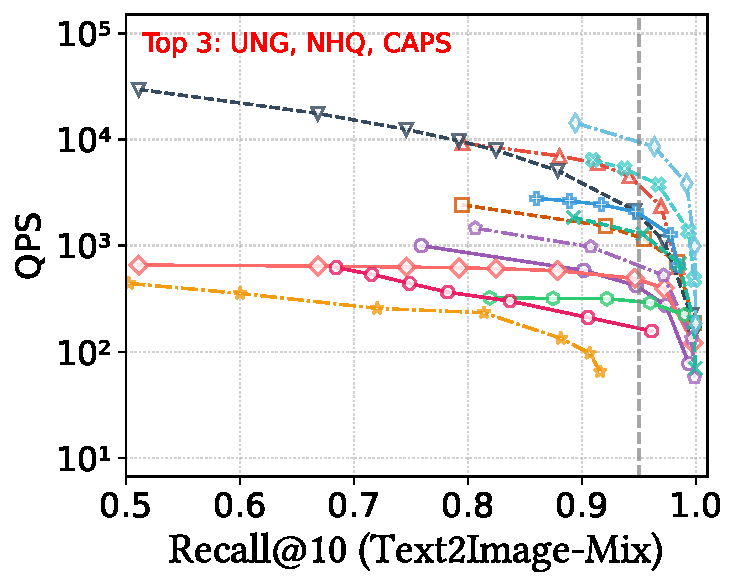
\includegraphics[width=\linewidth]{figures/exp/attribute_multimodel.pdf}
			\caption{\footnotesize MultiModel}
			\label{fig:rangeFilter_build_time}
		\end{subfigure}
		\hfill
		\begin{subfigure}[t]{0.315\columnwidth}
			\centering
			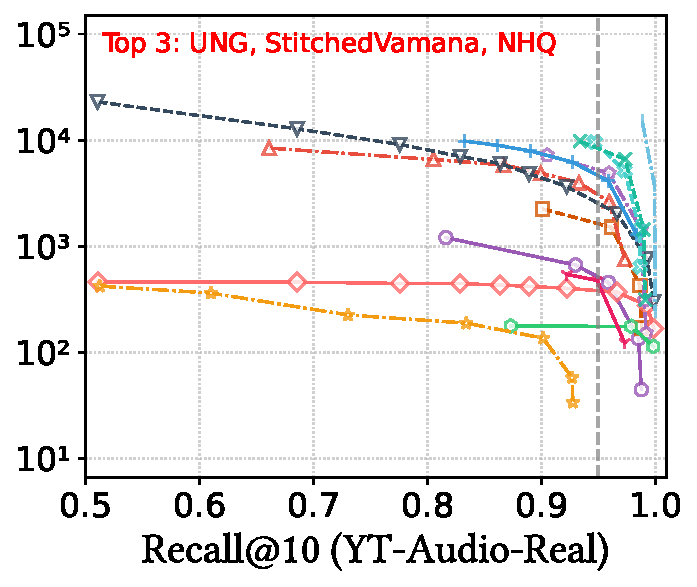
\includegraphics[width=\linewidth]{figures/exp/attribute_85.pdf}
			\caption{\footnotesize Different Computer}
			\label{fig:rangeFilter_index_size_mb}
		\end{subfigure}
		\hfill
		\begin{subfigure}[t]{0.315\columnwidth}
			\centering
			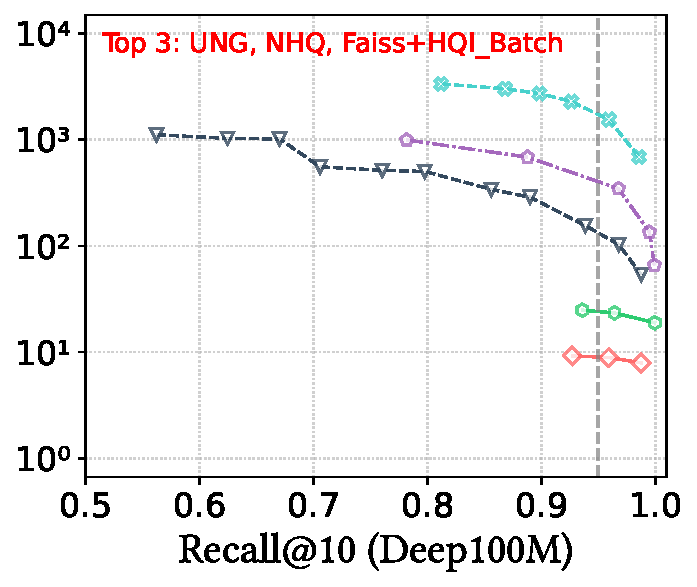
\includegraphics[width=\linewidth]{figures/exp/attribute_100M.pdf}
			\caption{\footnotesize Big Dataset}
			\label{fig:rangeFilter_build_memory_mb}
		\end{subfigure}

		
		\caption{\textcolor{violet}TrinityExtension——Attribution}
		\label{fig:TrinityExtension——Attribution}
	\end{figure}
	
	\subsection{Range Filtering}
	
	\subsubsection{Time and Space overhead of index construction.}
	
	\begin{figure}[t]
		\centering
		
		
		\hspace*{5pt}
		% 放大的图例(占满单栏)
		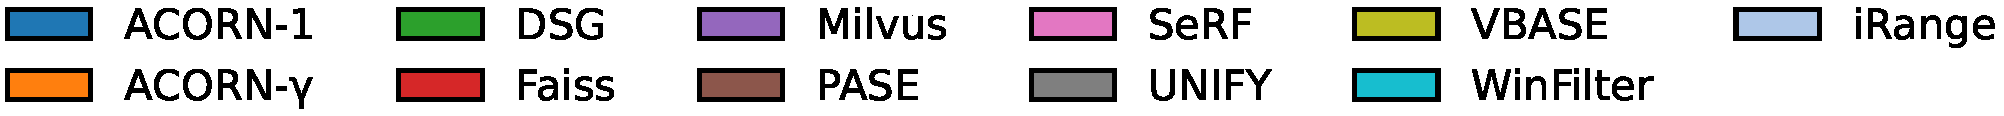
\includegraphics[width=0.98\columnwidth]{figures/indexData/rangeFilter_legend_only.pdf}
		
		%\vspace{0.1cm}
		
		% 三图横排
		\begin{subfigure}[t]{0.49\columnwidth}
			\centering
			\captionsetup{font=small}
			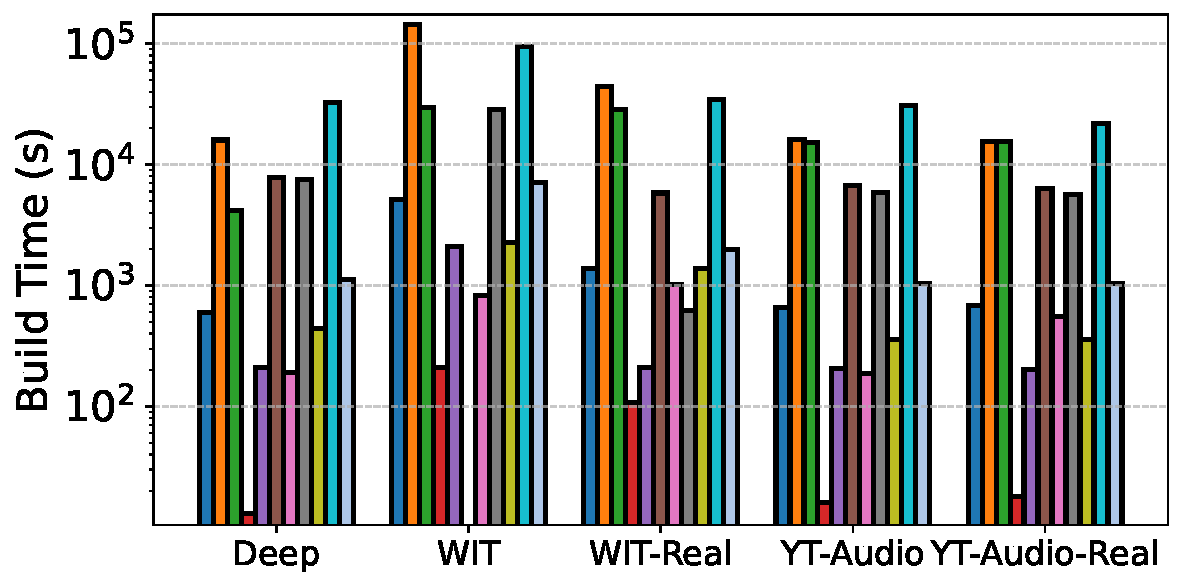
\includegraphics[width=\linewidth]{figures/indexData/rangeFilter_build_time_comparison_query.pdf}
			\caption{\footnotesize Construction time}
			\label{fig:rangeFilter_build_time}
		\end{subfigure}
		\hfill
		\begin{subfigure}[t]{0.49\columnwidth}
			\centering
			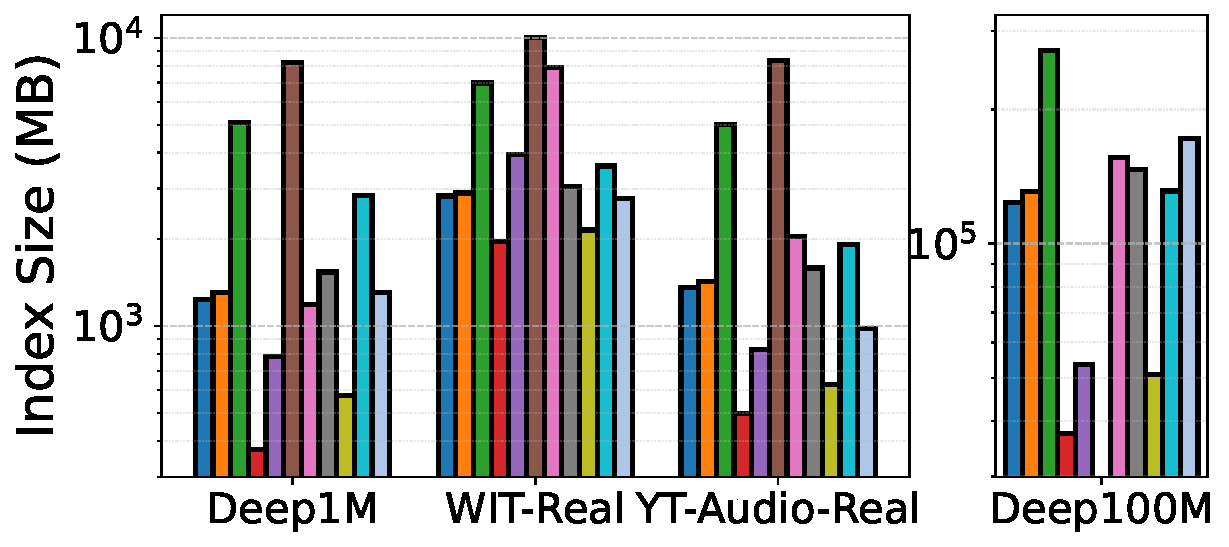
\includegraphics[width=\linewidth]{figures/indexData/rangeFilter_index_size_mb_comparison_query.pdf}
			\caption{\footnotesize Index size}
			\label{fig:rangeFilter_index_size_mb}
		\end{subfigure}
		\hfill
		\begin{subfigure}[t]{0.49\columnwidth}
			\centering
			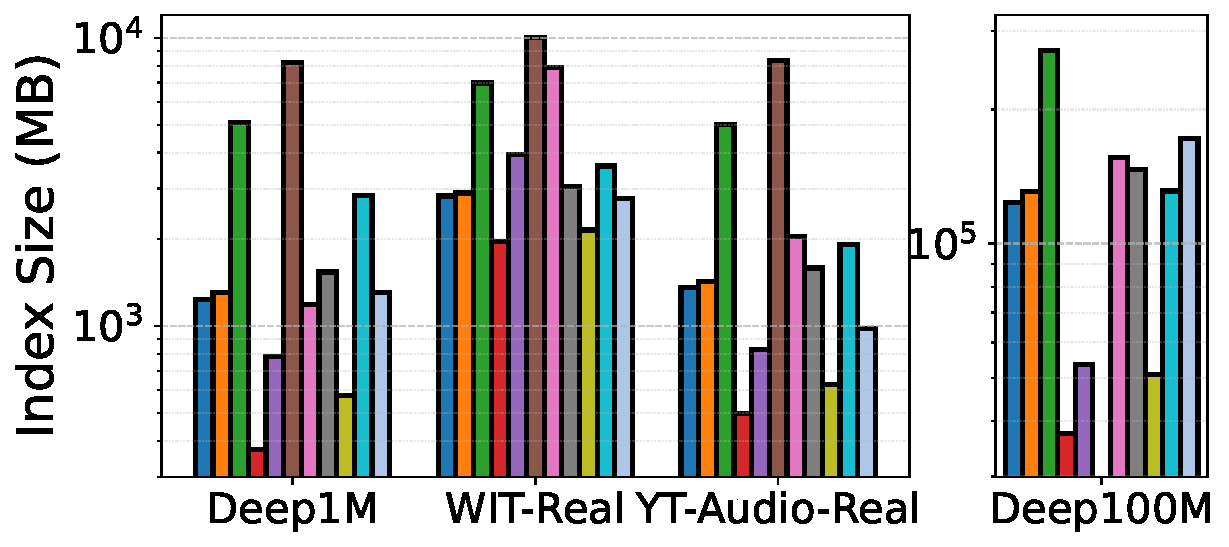
\includegraphics[width=\linewidth]{figures/indexData/rangeFilter_index_size_mb_comparison_query.pdf}
			\caption{\footnotesize Build peak memory}
			\label{fig:rangeFilter_build_memory_mb}
		\end{subfigure}
		\hfill
		\begin{subfigure}[t]{0.49\columnwidth}
			\centering
			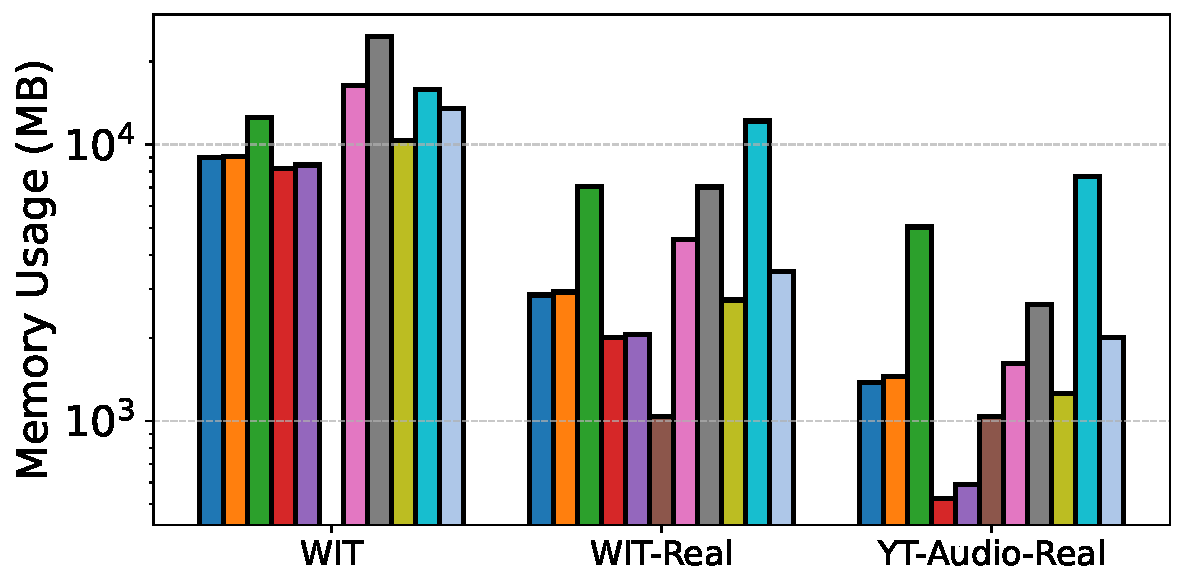
\includegraphics[width=\linewidth]{figures/searchMem/range_memory_comparison.pdf}
			\caption{\footnotesize Search peak memory}
			\label{fig:rangeFilter_search_memory_mb}
		\end{subfigure}
		
		%		\caption{Time and space overhead of range filtering index construction}
%		\caption{Time and space overhead of index construction}
		\caption{\textcolor{violet}{Time and space overhead}}
		\label{fig:rangeFilter_build_index_comparison}
	\end{figure}
	
	%Similar to the evaluation of \textit{Attribute Filtering} algorithms, 
	Similarly, we also evaluate 3 key metrics mentioned above in \textit{Range Filtering} algorithms.
	
	
	\textit{\textbf{Index construction time.}}
	Figure~\ref{fig:rangeFilter_build_time} shows the single-threaded index construction time. Faiss builds the index fastest. As Faiss obtains subsamples through sampling and calculates the cluster centroid, the computational complexity is significantly reduced.
	%	shows the single-threaded index construction time. Faiss builds the index fastest. Because Faiss obtains subsamples through sampling and then calculates the cluster centroid, the computational complexity is significantly reduced.
	
	
	WinFilter and ACORN-\(\gamma\) take the longest.
	WinFilter relies on a tree structure, requiring separate nearest-neighbor graphs per node. This causes redundant computation and high costs, especially for large datasets.
	ACORN-\(\gamma\) expands the neighbor list of each node to provide more candidate paths, which increases both computation and storage costs. It also prunes distant neighbors to save storage space. However, this introduces additional overhead and slows down the construction process.
	
	\textit{\textbf{Index size.}} 
	As shown in Figure~\ref{fig:rangeFilter_index_size_mb}, Among all algorithms, Faiss has the smallest index size. Because IVF only adds centroid data and partition information to the vector dataset, the IVF index is only slightly larger than the vector dataset.
	On low-dimensional datasets (Deep, YT-Audio), PASE requires the most storage. Its implementation likely wastes space due to alignment padding and inefficient encoding. %(e.g., Base64).
	
	SeRF maintains a compact index for low-dimensional data. However, for high-dimensional dataset (WIT), SeRF stores more edges and dynamic range data, significantly increasing its size.
	
	\textit{\textbf{Peak memory usage.}}
	As Figure~\ref{fig:rangeFilter_memory_mb} shows, Faiss uses the least memory on low-dimensional datasets. It stores minimal temporary data during index construction.
	
	On low-dimensional datasets, DSG and WinFilter exhibit higher peak memory usage compared to other algorithms. This suggests that their index structures suffer from severe structural redundancy and are difficult to compress in low-dimensional scenarios.
	%因为低维空间中数据点之间的欧氏距离普遍较小,点与点之间更易互为近邻,从而导致图索引中产生大量冗余的边连接。
	
	
	%As Figure~\ref{fig:rangeFilter_memory_mb} shows, Faiss uses the least memory on low-dimensional datasets (Deep, YT-Audio). It stores minimal temporary data (e.g., vectors, centroids, distances) during index construction.
	
	For high-dimensional dataset WIT, iRange achieves the lowest peak memory usage. It pre-builds graphs only for a limited number of intervals, avoiding explicit index construction for all possible query ranges. Its index structure remains stable in high dimensions without significant graph growth. This effectively controls index size, making iRange more advantageous for high-dimensional datasets.
	In contrast, Unify exhibits the highest memory consumption, indicating that its index construction process is highly sensitive to the dimensionality of the data.
	
	\begin{figure*}[t]
		
		\centering
		
		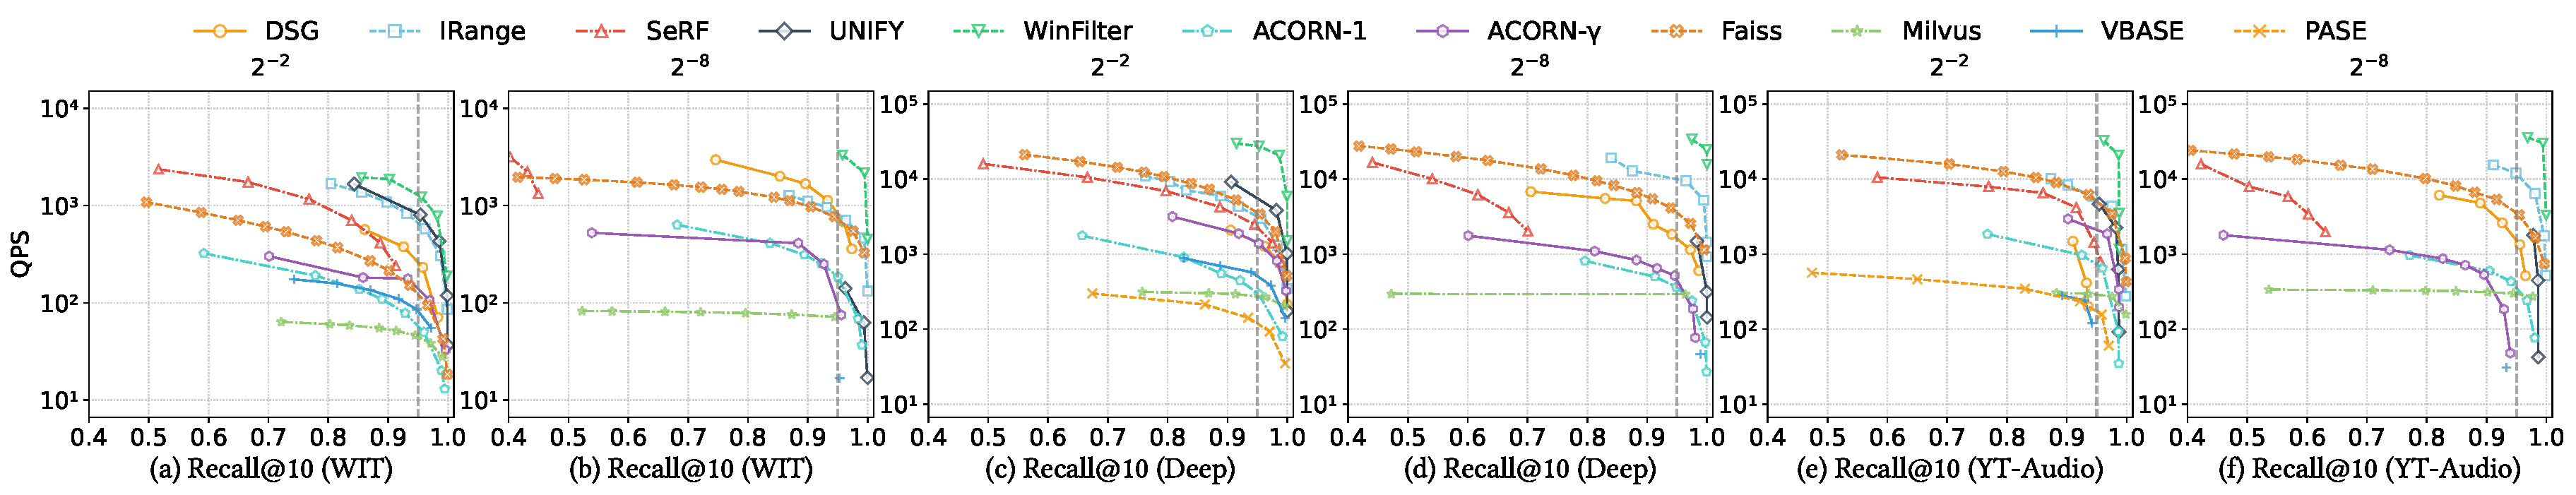
\includegraphics[width=0.92\textwidth]{figures/exp/exp_8_2.pdf}
		\caption{RF-ANN search }
		\label{fig:exp_8_2}
	\end{figure*}
	
	
	\subsubsection{Performance Evaluation. }
	
	In this experiment, we follow the query range definition adopted by prior work~\cite{HQI}. Specifically, for a given query, if the range covers $n/2^i$ data points—where $n$ is the total dataset size—we define the range ratio as $2^{-i}$. Based on this definition, we evaluate algorithm performance under 4 query range settings: $2^{-2}$, $2^{-4}$, $2^{-6}$, and $2^{-8}$.
	
	Due to space constraints, Figure~\ref{fig:exp_8_2} reports results for only the largest ($2^{-2}$) and smallest ($2^{-8}$) range ratios. The experimental results show that across all datasets (Deep, YT-Audio, and WIT) and query ranges, WinFilter consistently delivers the best performance. This highlights its robustnes, which performs ANN search over only relevant tree nodes and merges results efficiently, making it highly effective for static range query scenarios.
	
	iRange offers a good balance between query efficiency and recall, demonstrating stable performance across both datasets and range sizes. In contrast, UNIFY experiences a notable drop in performance under narrow query ranges, suggesting that its HSIG structure—despite incorporating skip lists for pre-filtering—still has limitations in such scenarios. However, by leveraging HNSW and bitmap-based post-filtering, UNIFY performs competitively under broader range conditions, demonstrating strong scalability.
	
%	SeRF exhibits relatively weak overall performance, with a significant drop in recall under small-range query scenarios. This suggests that while its compressed graph structure is space-efficient, it has a substantial negative impact on query performance.

	\textcolor{blue}{SeRF demonstrates relatively weak overall performance, with a pronounced drop in recall under small-range query scenarios. This is because SeRF compresses the entire HNSW graph by attaching range information to its edges. However, during small-range queries, its multi-filtering mechanism requires scanning a large number of edge entries that are irrelevant to the current query range, introducing fixed computational and memory access overhead. Additionally, graph traversal may lead to the exploration of numerous invalid neighbors, increasing the likelihood of the search becoming trapped in local optima and further degrading performance.
	}
	
	%	 修改此处
	ACORN performs similarly on both large and small range queries, but its overall performance is worse than the other methods. Unlike other range filtering algorithms, ACORN is not designed with specialized data structures  to achieve efficient range filtering. In fact, the graph structure used by ACORN for attribute filtering is the same as that used for range filtering.
	
	For third-party library and databases, Figure~\ref{fig:exp_8_2} shows that Faiss performs well in range filtering and even outperforms some specialized range query algorithms in certain cases. 
	%\textcolor{blue}{since attributes are pre-sorted in range filtering scenarios, the filtering overhead is minimal, leading to improved query performance. Similar to the selectivity observed in attribute filtering. }
	Faiss performs better in small-range filtering scenarios because it searches over the filtered vectors. With a smaller range, fewer points remain after filtering, resulting in lower computational cost. In addition, the performance of Faiss is influenced by data dimensionality; the higher the dimensionality, the worse the performance.
	
	Vector databases also show relatively poor performance on range queries. Among them, Milvus performs more balanced across both small-range and large-range queries, even surpassing ACORN under high recall settings. PASE performs poorly on small-range queries, with recall lower than 0.1, due to its post-filtering strategy. 
	VBASE performs moderately; it works well for large-range queries, but for small-range queries, although it achieves high recall, its QPS is quite  low.
	
	
	
	It is important to note that this range query experiment is conducted under a fully static setting. Under such conditions, UNIFY, iRange, SeRF, and WinFilter require the dataset to be sorted by attribute prior to index construction. In contrast, DSG  supports dynamic index construction with unordered attribute insertions, making it more suitable for streaming or incremental data scenarios. This flexibility highlights its superior extensibility in real-world applications.
	\subsubsection{Robustness.}
	
	
	\begin{figure*}[htbp]
		\centering
		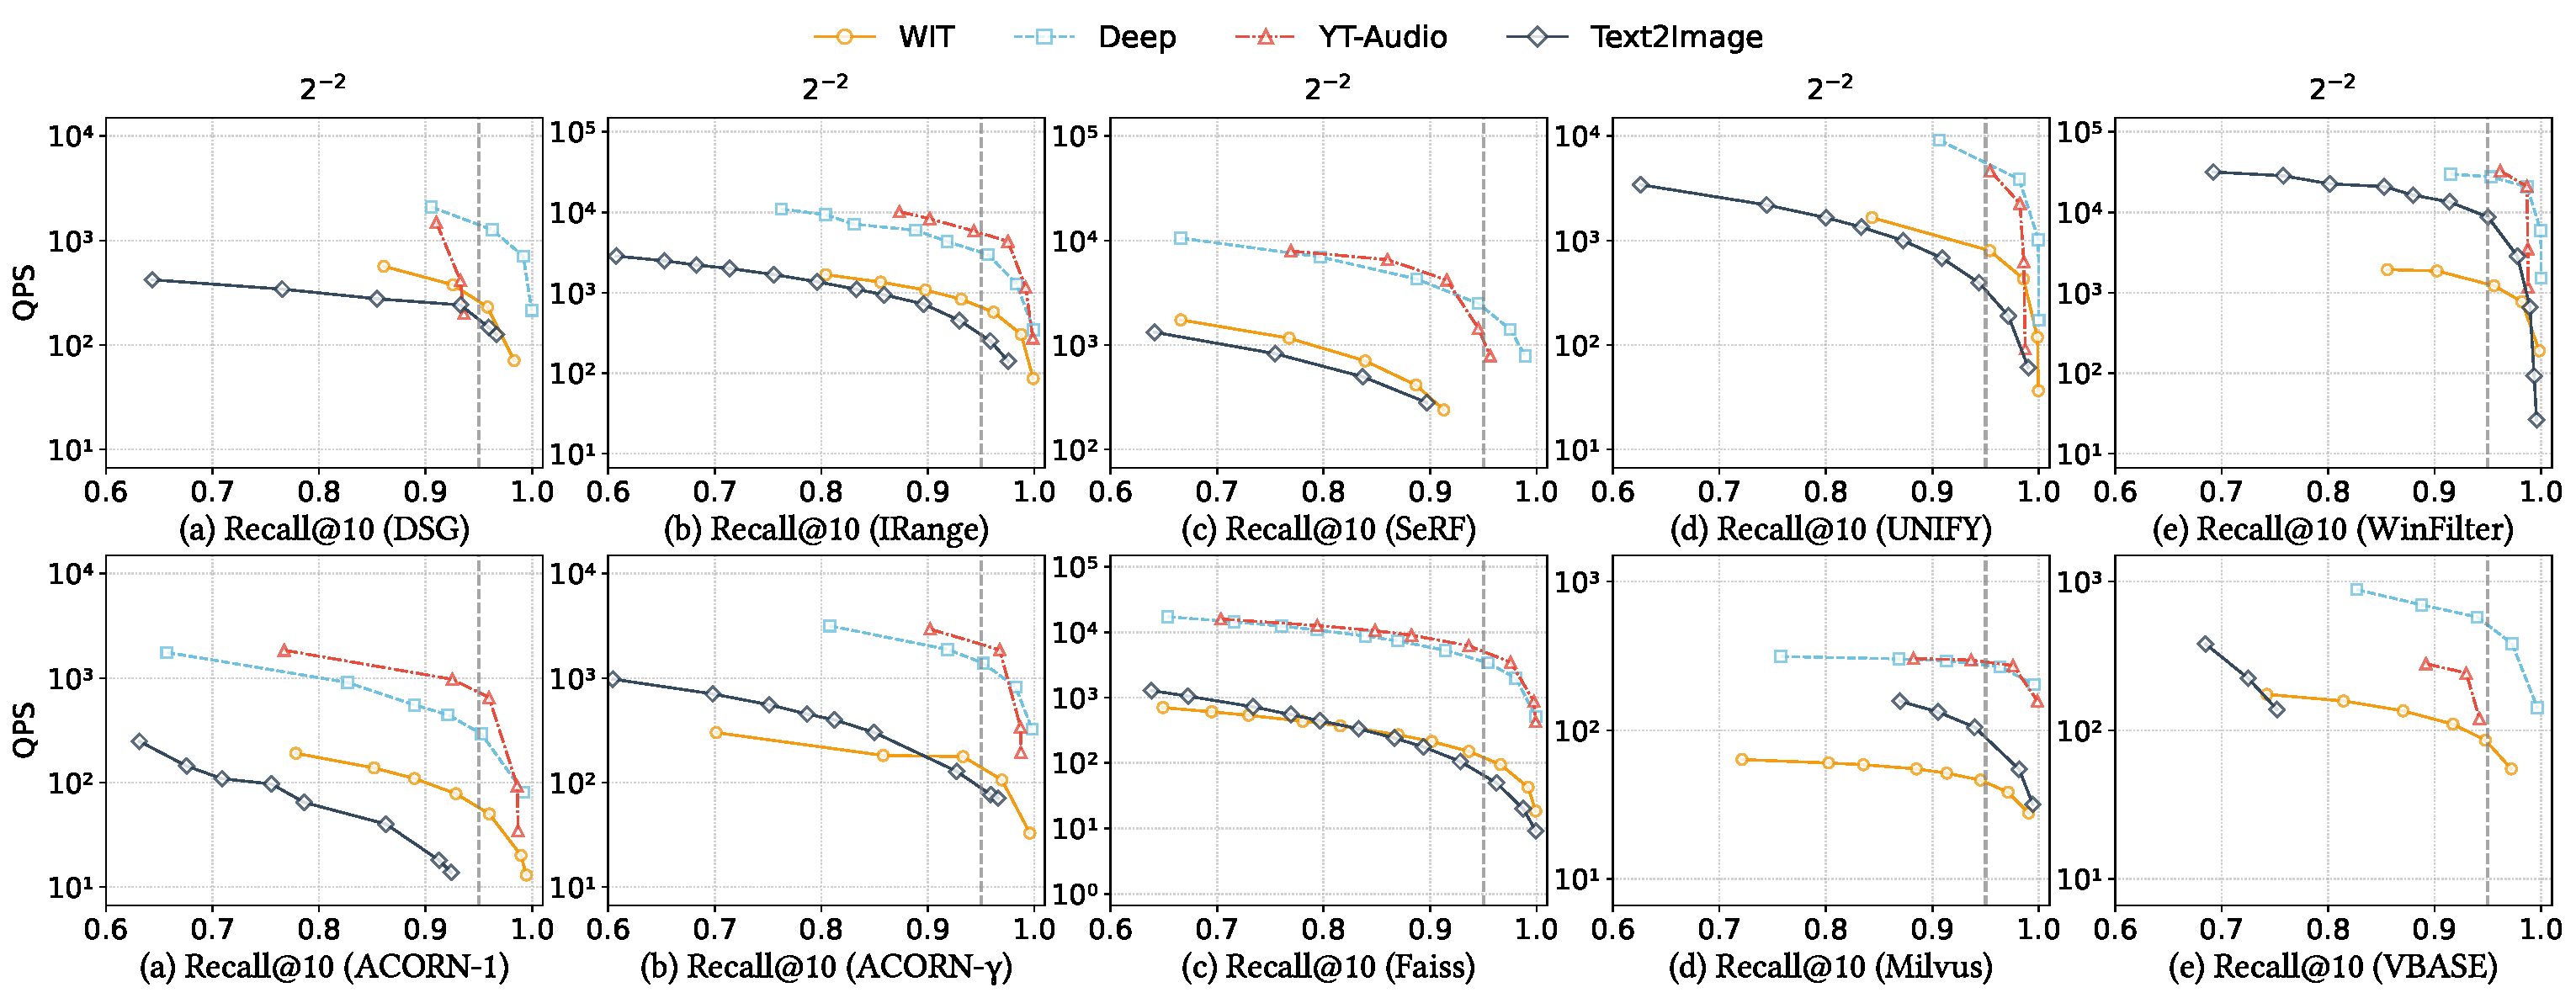
\includegraphics[width=0.80\textwidth]{figures/exp/exp_8_3.pdf}
		\caption{Dataset Effect on RF-ANN Search}
		\label{fig:exp_8_3}
	\end{figure*}
	
	To evaluate the robustness of the RF-ANNS algorithms in different scenarios, we add an OOD dataset in the experiments. As shown in Figure~\ref{fig:exp_8_3}, most methods perform worst on the Text2Image dataset. This is because OOD queries make the $k$-nearest neighbor distribution more sparse. As a result, the search needs to visit more nodes, which leads to an exponential growth in the search space and a sharp drop in efficiency.
	
	WinFilter shows the worst performance on the WIT dataset. This suggests that its performance is sensitive to the data dimensionality. ACORN has large performance differences across datasets, indicating weak robustness.
	
	Among vector databases, Milvus performs well. VBASE is sensitive to datasets and achieved recall below 0.8 on Text2Image. PASE is excluded from this round of tests because it does not support datasets with dimensions over 512 and performed poorly in earlier experiments.
	
	It is worth noting that most methods achieve similar performance on the Deep and YT-Audio datasets, which have similar LID values. This shows that RF-ANNS performance is largely affected by both the LID and the dimensionality of the dataset. A high LID and high dimensionality make hybrid queries more difficult.
	
	However, even though Deep and YT-Audio have similar LID values, the DSG algorithm shows large performance differences between them. This means that DSG is more sensitive to changes in data distribution. 
	%	Its robustness is lower than that of other methods, possibly because it depends not only on LID but also on other complex data characteristics.
	%	To examine the robustness of RF-ANNS algorithms, we analyze their performance across different datasets. As shown in Figure~\ref{fig:exp_8_3}, the performance differences. All methods perform worst on WIT, which has the highest LID. On Deep and YT-Audio, which have similar LID, most algorithms achieve comparable performance. 
	%	This suggests that the effectiveness of RF-ANN search is mainly influenced by LID of the dataset. A higher LID inherently increases the difficulty of hybrid query.
	%	
	%	However, the DSG algorithm shows a noticeable performance gap between the Deep and YT-Audio datasets, despite their comparable LID. This indicates that DSG is less robust than other methods when facing dataset-dependent variations, possibly due to its sensitivity to data distribution beyond LID alone.
	\textit{\textbf{Multimodel, 85 and Deep100M.}} \textcolor{red}{The fig is Figure \ref{fig:TrinityExtension——Range}}
	
	\begin{figure}[t]
		\centering
		
		
		\hspace*{5pt}
		% 放大的图例(占满单栏)
		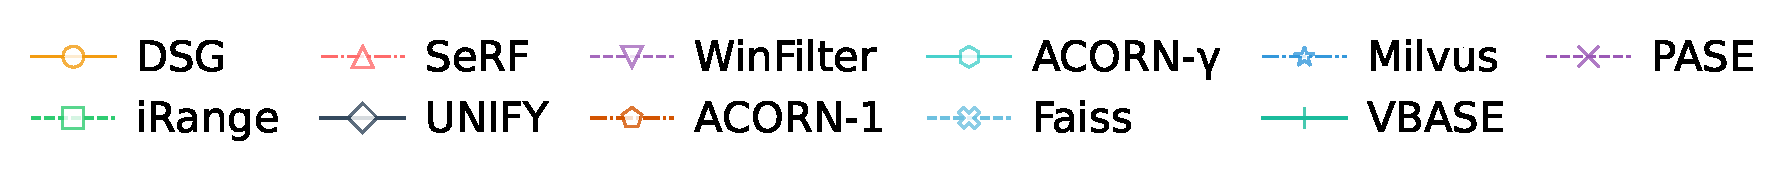
\includegraphics[width=0.98\columnwidth]{figures/exp/range_legend.pdf}
		
		%\vspace{0.1cm}
		\begin{subfigure}[t]{0.332\columnwidth}
			\centering
			\captionsetup{font=small}
			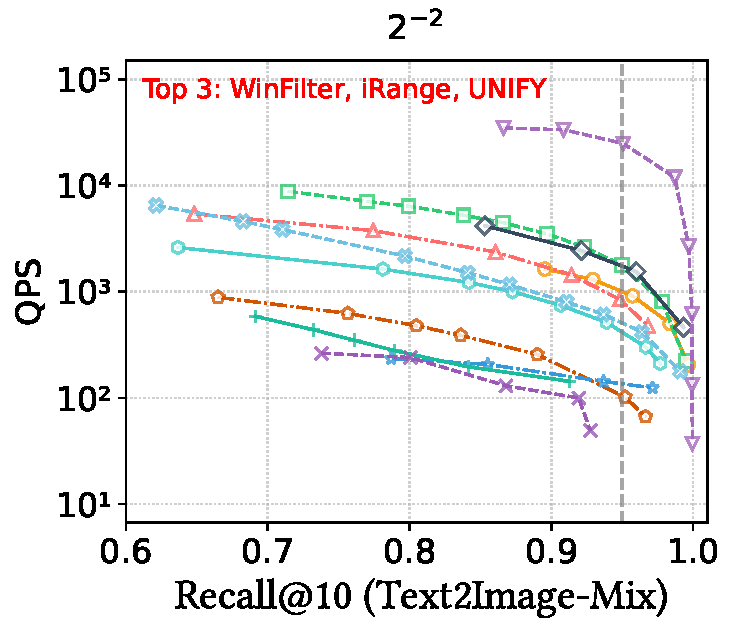
\includegraphics[width=\linewidth]{figures/exp/range_multimodel.pdf}
			\caption{\footnotesize MultiModel}
			\label{fig:MultiModel range}
		\end{subfigure}
		\hfill
		\begin{subfigure}[t]{0.315\columnwidth}
			\centering
			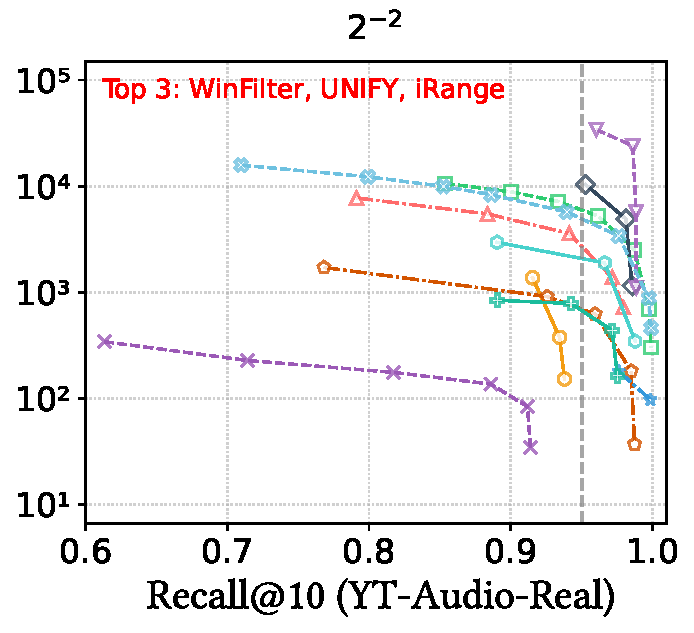
\includegraphics[width=\linewidth]{figures/exp/range_85.pdf}
			\caption{\footnotesize Different Computer}
			\label{fig:Different Computer range}
		\end{subfigure}
		\hfill
		\begin{subfigure}[t]{0.315\columnwidth}
			\centering
			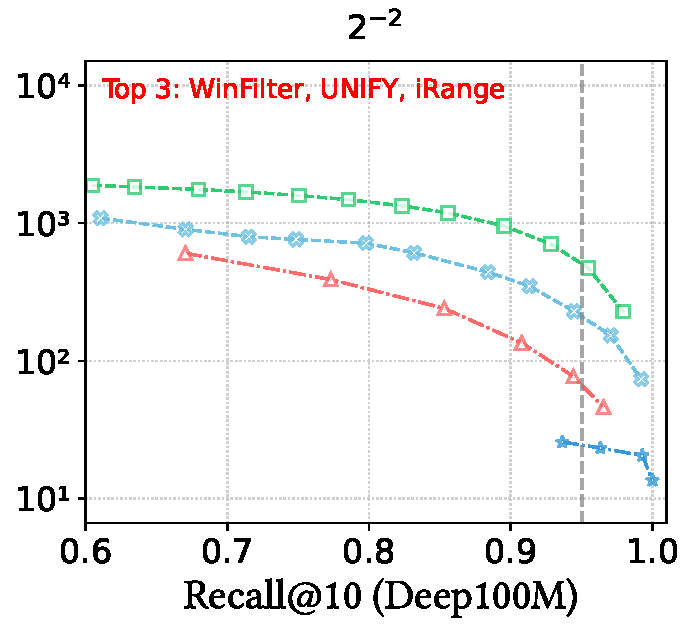
\includegraphics[width=\linewidth]{figures/exp/range_deep100M.pdf}
			\caption{\footnotesize Big Dataset}
			\label{fig:Big Dataset range}
		\end{subfigure}
		
		
		\caption{\textcolor{red}TrinityExtension——Range}
		\label{fig:TrinityExtension——Range}
	\end{figure}
	
	
	\section{DISCUSSION}
	Based on the performance of the algorithms on different experimental scenarios, we discuss our findings as follows.
	
	
	\subsection{Recommendations.}
	%Based on the performance of different algorithms in experiments, we recommend algorithms suitable for different scenarios, as shown in the table \ref{tab:algo_scenarios}.
	
	
	\begin{table}[t]
		\centering
		
		\caption{Algorithm Recommendation per Scenario}
		\resizebox{\columnwidth}{!}{
			\begin{tabular}{|l|c|c|}
				\hline
				\textbf{Scenario} & \textbf{Attribute Filtering} & \textbf{Range Filtering}\\
				\hline
				S1: Large-scale Datasets & Puck, UNG & iRange\\[1pt]
				\hline
				S2: Fast Index Construction & ACORN-1, UNG  &Faiss\\[1pt]
				\hline
				S3: Query on Hard Datasets & CAPS, UNG &WinFilter, iRange, DSG\\[1pt]
				\hline
				S4: Query on Easy Datasets & StitchedVamana, NHQ, UNG & WinFilter, iRange\\[1pt]
				
				\hline
				S5: General-purpose Use & Milvus, Faiss &DSG, UNIFY\\[1pt]
				\hline
				S6: Resource constraint& CAPS, Faiss&Faiss, SeRF \\[1pt]
				\hline
				S7: High-Recall Querying & UNG & WinFilter \\[1pt]
				\hline
				S8: OOD scenarios & UNG &WinFilter  \\[1pt]
				\hline
			\end{tabular}
		}
		\label{tab:algo_scenarios}
	\end{table}
	
	\subsubsection{\textbf{Attribute Filtering}}
	We summarize the applicability of different algorithms across various attribute filtering scenarios in Table~\ref{tab:algo_scenarios}. Puck and UNG excel on large-scale datasets (S1). ACORN-1 and UNG achieve fast index construction (S2). UNG performs well on different datasets (S3, S4). In addition, CAPS performs well on hard datasets with high LID (S3), while NHQ and StitchedVamana perform better on easy datasets with low LID (S4).
	Faiss and CAPS can generate relatively compact indexes with low memory usage, which is suitable for resource-constrained situations (S6). Milvus and Faiss serve as general-purpose solutions (S5). UNG stands out for its higher recall, precision, and QPS, and performs well in the OOD scenario (S7, S8).
	\subsubsection{\textbf{Range Filtering}}
	
	Table~\ref{tab:algo_scenarios} also shows the application scenarios of range filtering. iRange performs well on large-scale datasets, combining efficient construction and excellent query capabilities (S1). Faiss performs well in fast index construction (S2). When processing hard datasets, WinFilter, iRange, and DSG are recommended (S3), while WinFilter and iRange also perform well on easy datasets (S4). For general applications, DSG supports dynamic updates, while UNIFY provides flexible filtering strategies (S5). Faiss and SeRF show superior memory efficiency (S6). For static queries with high recall, WinFilter is the best choice (S7). In addition, WinFilter also performs well in OOD scenarios (S8).
	\subsection{Challenges}
	\subsubsection{\textbf{Attribute Filtering}}
	Most existing attribute filtering algorithms are graph-based, they typically outperform other methods in terms of query accuracy and efficiency. Filtered-DiskANN leverages disk-based storage, making it more suitable for extremely large-scale datasets even in memory-constrained environments. Moreover, the index construction phase of graph-based algorithms is computationally intensive. Therefore, exploring GPU-based acceleration for graph construction and vector computation during indexing is promising. It can significantly improve the performance of graph-based methods.
	
	Furthermore, current attribute filtering algorithms offer limited support for complex filtering conditions. For example, Filtered-DiskANN  supports single-attribute filtering, and in multi-attribute scenarios, it only supports OR conditions between attributes. 
	%The original implementations of 
	NHQ imposes strict constraints on the number of base and query attributes and only support AND conditions. While UNG is relatively flexible—supporting both AND and OR logic—it still lacks support for arbitrary Boolean expressions (e.g., combinations of AND and OR). The lack of flexible Boolean filtering remains a key challenge, limiting the practicality of hybrid query methods in real-world systems with diverse and complex query requirements.
	
	\subsubsection{\textbf{Range Filtering}}
	
	Except for DSG, most range filtering algorithms require the dataset to be pre-sorted before building the index. Moreover, these methods do not support multi-attribute range queries. Enhancing these methods to support an arbitrary number of range filterable attributes remains an open research challenge.
	
	Our experiments show that graph compression methods often lead to poor query performance in RF-ANN search. To address this problem, subsequent algorithms usually optimize the index processing at the segment tree nodes. UNIFY newly proposes segment graphs and integrates multiple data structures to process queries. Although UNIFY performs slightly worse on small-range queries, its proposed index structure broadens the research direction.
	
		In our experiments, many range filtering algorithms perform worse than Faiss at high recall (0.95), showing that current algorithm designs still need improvement. We suggest future future range filtering algorithms include Faiss as a baseline.
		%In our experiments, we find that many range filtering algorithms perform worse than Faiss at high recall (0.95). This shows that the design of current algorithms still needs improvement. We suggest that future range filtering algorithms should include Faiss as a baseline.
	
	
	It is also worth noting that range filtering and attribute filtering are both forms of hybrid query. However, aside from vector databases and ACORN, few existing algorithms support both modalities simultaneously. Designing unified frameworks that simultaneously support both is an important research frontier. 
	
	Lastly, our findings show that the distribution and the number of attributes, as well as dataset properties (e.g., dimensionality and LID), significantly impact the performance of attribute filtering methods. Enhancing the robustness of these algorithms under diverse data conditions is another key challenge that warrants further investigation.
	
	
	\section{CONCLUSION}
	In this paper, we systematically evaluate hybrid query methods, including various algorithms, vector databases, and libraries. We enrich the attribute information of the dataset and design a variety of experimental scenarios, and comprehensively analyze the performance of each algorithm. Experiments show that these algorithms still have shortcomings in scenarios such as large-scale data, complex queries, and resource constraints. There are still significant deficiencies in the flexibility and Boolean logic support of attribute filtering algorithms. Additionally, the performance of range filtering algorithms remains limited under high-recall requirements and lacks support for multi-attribute queries. Notably, some algorithms even perform worse than the baseline method (e.g., Faiss) in high recall scenarios.  In the future, it is essential to further explore the flexibility and robustness of attribute filtering algorithms, and improving the performance of range filtering algorithms remains an important direction.
%	\textcolor{blue}{
%		In this paper, we evaluate hybrid query methods, including algorithms, vector databases, and libraries. We design experiments to assess the performance of attribute filtering algorithms. We enrich existing datasets with attribute values and create various experimental scenarios to ensure fair comparisons. We run experiments on 7 real-world datasets to analyze the effectiveness of attribute filtering algorithms. We also compare range filtering algorithms using 4 range query datasets. Finally, we analyze the results, summarize key findings, and identify areas for improvement. Our study validates previous research and provides insights for future work.
%	}
%	
	
	
	
	\clearpage
	
	\bibliographystyle{ACM-Reference-Format}
	\bibliography{sample}
	%\end{sloppypar}
\end{document}
\endinput